\documentclass[11pt]{article}

% ---------------------------------------------------------------- packages
\usepackage[T1]{fontenc}
\usepackage{lmodern}
\usepackage[margin=1in]{geometry}
\usepackage{microtype}
\usepackage{amsmath,amssymb,bm}
\usepackage{graphicx}
\usepackage{booktabs,tabularx,multirow,array,makecell}
\usepackage{enumitem}
\usepackage{xcolor}
\usepackage[font=small,labelfont=bf]{caption}
\usepackage{tikz}
\usetikzlibrary{positioning,arrows.meta,shapes.geometric,fit,calc,backgrounds}
\usepackage[edges]{forest}
\usepackage[
  backend=biber,
  style=authoryear-comp,
  maxcitenames=2,
  mincitenames=1,
  maxbibnames=8,
  minbibnames=6,
  uniquelist=false,
  uniquename=false,
  giveninits=true,
  doi=true,
  url=false,
  isbn=false,
  eprint=true,
  dashed=false,
  sorting=nyt
]{biblatex}
\addbibresource{references.bib}
\DeclareFieldFormat[article,inproceedings,incollection,misc]{title}{#1}
\renewbibmacro{in:}{\ifentrytype{article}{}{\printtext{\bibstring{in}\intitlepunct}}}
\usepackage[colorlinks=true,linkcolor=linkblue,citecolor=linkblue,urlcolor=linkblue]{hyperref}
\usepackage[capitalise,nameinlink]{cleveref}

% ------------------------------------------------------------------ colors
% Categorical slots shared with the Python figures (code/style.py).
\definecolor{linkblue}{HTML}{1C5CAB}
\definecolor{cblue}{HTML}{2A78D6}
\definecolor{corange}{HTML}{EB6834}
\definecolor{caqua}{HTML}{1BAF7A}
\definecolor{cviolet}{HTML}{4A3AA7}
\definecolor{cmagenta}{HTML}{E87BA4}
\definecolor{cink}{HTML}{0B0B0B}
\definecolor{cink2}{HTML}{52514E}
\definecolor{cneutral}{HTML}{F0EFEC}

% ------------------------------------------------------------ float setup
\renewcommand{\topfraction}{0.9}
\renewcommand{\bottomfraction}{0.8}
\renewcommand{\textfraction}{0.07}
\renewcommand{\floatpagefraction}{0.75}
\setcounter{topnumber}{3}
\setcounter{totalnumber}{4}
\setlength{\emergencystretch}{1.5em}

% ---------------------------------------------------------------- notation
\newcommand{\R}{\mathbb{R}}
\newcommand{\q}{\bm{q}}
\newcommand{\z}{\bm{z}}
\newcommand{\X}{\bm{X}}
\newcommand{\W}{\bm{W}}
\newcommand{\Phib}{\bm{\Phi}}
\newcommand{\enc}{\mathcal{E}}
\newcommand{\dec}{\mathcal{D}}
\newcommand{\M}{\mathcal{M}}
\DeclareMathOperator*{\argmin}{arg\,min}
\DeclareMathOperator{\spn}{span}

\title{\textbf{Dimensionality Reduction for Machine Learning\\ in Fluid Dynamics: A Review}}
\author{Caleb A. Morton\\[2pt]
  \small Department of Mechanical \& Aerospace Engineering, The Ohio State University}
\date{\today}

\begin{document}
\maketitle

\begin{abstract}
\noindent
High-fidelity simulations and time-resolved measurements of fluid flows produce
state vectors with $10^{5}$--$10^{9}$ degrees of freedom, yet the dynamics they
record are often confined to far fewer effective coordinates. Nearly every
machine-learning model of a fluid system therefore begins by compressing the flow
into a low-dimensional representation, and the choice of that representation
limits what the downstream model can learn. This review surveys dimensionality
reduction from a fluid-dynamics perspective, covering four families.
Linear modal decompositions include proper orthogonal decomposition, dynamic
mode decomposition, and their spectral and balanced variants.
Sparse, clustered, and spatially localized representations include domain
decomposition, generalized finite element enrichment, and data-informed local
subspaces. Nonlinear manifold learning is covered in both its kernel and graph
forms and its neural-network form: autoencoders, variational autoencoders, graph
autoencoders, and implicit neural representations. The last family is
operator-learning architectures whose latent spaces play the same role. For
each family we summarize the mathematical formulation, the properties that
matter for learning dynamics, and representative fluid applications. We then
examine how reduced coordinates are coupled to learned dynamics, including
Galerkin and operator-inference models, sparse regression, Koopman embeddings,
recurrent and attention-based sequence models, and latent generative models. We
also discuss what makes a latent space good for forecasting rather than
reconstruction alone. Computed examples on a lid-driven cavity at
$\mathrm{Re}=15{,}000$ and on canonical transport problems illustrate the main
trade-offs, including the Kolmogorov $n$-width barrier, the accuracy ceiling of
learned nonlinear decoders, and the effect of spatial localization. We close
with a comparative assessment, recommendations on baselines and metrics, and
open challenges for high-Reynolds-number, three-dimensional, and
parametrically varying flows.
\end{abstract}

\tableofcontents
\newpage

% ======================================================================
\section{Introduction}
\label{sec:intro}
% ======================================================================

\subsection{Why reduce dimension before learning?}

Turbulent and transitional flows are governed by partial differential equations
whose discretizations carry an enormous number of degrees of freedom. A direct
numerical simulation must resolve length scales from the integral scale down to
the Kolmogorov scale, and the number of grid points grows roughly as
$\mathrm{Re}^{9/4}$ for homogeneous turbulence \parencite{pope2000turbulent}.
Time-resolved particle image velocimetry (PIV) and large-eddy simulations of
engineering configurations likewise produce terabytes of spatio-temporal data.
Yet the dynamics recorded in these data are rarely as complex as their
dimension suggests. Coherent structures, symmetries, and dissipation confine
the long-time behavior of many flows to a comparatively thin subset of state
space. For dissipative systems this subset is sometimes formalized as an
\emph{inertial manifold} \parencite{foias1988inertial}, and more generally it
is the fluid-dynamical instance of the \emph{manifold hypothesis} that
underlies much of modern representation learning
\parencite{bengio2013representation,fefferman2016manifold}.

Dimensionality reduction (DR) exploits this structure by constructing a map
from the high-dimensional flow state to a small set of coordinates, and
usually also a map back. In fluid mechanics DR has served three overlapping
purposes. \emph{Analysis:} modal decompositions reveal coherent structures and
their frequencies \parencite{taira2017modal,taira2020modal}. \emph{Modeling:}
projection-based reduced-order models (ROMs) evolve a few modal amplitudes in
place of the full field \parencite{holmes2012turbulence,benner2015survey,rowley2017arfm}.
\emph{Learning:} most machine-learning (ML) models of fluid systems operate in a
compressed latent space because learning directly on the full state is
statistically and computationally prohibitive
\parencite{brunton2020ml,vinuesa2022enhancing,brunton2024promising}. This
review is concerned primarily with the third role, which inherits its
vocabulary and many of its tools from the first two.

The reasons to reduce dimension before learning are practical as well as
conceptual. Many-query tasks such as design optimization, uncertainty
quantification, control, and real-time simulation require thousands of
evaluations, which is exactly where surrogate models are valuable
\parencite{benner2015survey}. A learned model on a compact latent space has
fewer parameters, trains on far fewer samples, and can be rolled out
autoregressively at negligible cost. The latent coordinates can also be chosen
to make the downstream problem easier: approximately linear
\parencite{lusch2018koopman}, sparse in a function library
\parencite{champion2019sindyae}, statistically disentangled
\parencite{eivazi2022betavae,solera2024betavae}, or spatially local
\parencite{deshmukh2020dls,morton2026scitech}. The representation fixes an
upper bound on the fidelity of any model built on it. Features the encoder
discards cannot be recovered by the dynamics model, and features that are
represented in a tangled or temporally rough way make the forecasting problem
harder. Understanding the available DR techniques, and their consequences for
learning, is therefore a prerequisite for building reliable data-driven models
of fluid flows.

\subsection{Scope and relation to existing reviews}

Several excellent reviews cover parts of this landscape. Modal analysis of
fluid flows is surveyed by \textcite{taira2017modal,taira2020modal}, and the
theory of proper orthogonal decomposition (POD) by \textcite{berkooz1993} and
\textcite{holmes2012turbulence}, and textbook treatments of data-driven
modeling and reduced-basis methods are given by \textcite{brunton2019data} and
\textcite{hesthaven2016certified}. Projection-based model reduction is reviewed by
\textcite{benner2015survey}, \textcite{rowley2017arfm},
\textcite{lassila2014mor}, and \textcite{hesthaven2022acta}, and intrusive and
non-intrusive ROMs are surveyed briefly by \textcite{padula2024brief}. Closure modeling
is reviewed by \textcite{ahmed2021closures}. Machine learning for fluid
mechanics more broadly is reviewed by \textcite{brunton2020ml},
\textcite{duraisamy2019turbulence}, \textcite{vinuesa2022enhancing},
\textcite{vinuesa2024perspectives}, and \textcite{brunton2024promising}.
Operator inference is reviewed by \textcite{kramer2024opinf}. Closest in
spirit to the present article is the tutorial of \textcite{mendez2023linear},
which connects linear and nonlinear DR from fluid mechanics to ML, together
with the comparative study of \textcite{csala2022comparing}.

The present review differs in three ways. First, it is organized around the
\emph{use} of reduced coordinates in learning pipelines, so it treats encoder
design and latent dynamics jointly and emphasizes the properties of a latent
space that matter for forecasting. Second, it gives explicit attention to
\emph{spatially localized} representations, from domain-decomposed reduced
bases to generalized finite element enrichment and data-informed local
subspaces (DLS) \parencite{deshmukh2020dls}. These have received less attention
in the ML literature than global modal and autoencoder bases, yet they address
directly the multi-scale character of high-Reynolds-number turbulence. Third,
it includes computed examples that make the central trade-offs concrete: the
Kolmogorov $n$-width of transport problems, the accuracy ceiling of learned
nonlinear decoders, and the effect of localization on a turbulent cavity flow.
We restrict attention to reduction of the \emph{state} (the flow field). Sensor
placement, super-resolution, and closure modeling are mentioned only where they
bear directly on representation.

\subsection{Organization}

\Cref{fig:timeline} places the methods discussed here on a common timeline,
grouped into five families that also structure the article.
\Cref{sec:formulation} introduces notation, defines what is meant by a good
reduced representation, and presents a taxonomy.
\Cref{sec:linear} reviews linear subspace methods and their limitations, and
\cref{sec:local} reviews sparse, clustered, and spatially localized
representations, including DLS. \Cref{sec:manifold} covers classical
(non-neural) manifold learning, and \cref{sec:autoencoders} covers neural
autoencoders. \Cref{sec:meshfree} discusses graph-based, mesh-agnostic, and
operator-learning representations. \Cref{sec:dynamics} examines how reduced
coordinates are coupled to learned dynamics. \Cref{sec:assessment} provides a
comparative assessment with recommendations on baselines and metrics, and
\cref{sec:outlook} outlines open challenges.

\begin{figure}[tbp]
  \centering
  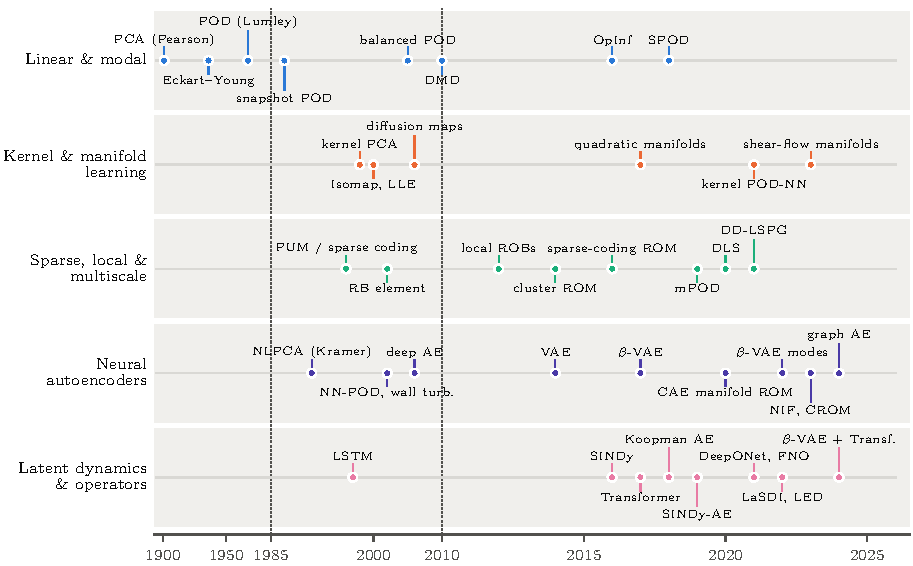
\includegraphics[width=\textwidth]{figs/timeline.pdf}
  \caption{Selected developments in dimensionality reduction relevant to fluid
  dynamics, grouped by family. The time axis is piecewise linear, with changes
  of scale at 1985 and 2010 (dashed lines). Representative references:
  PCA \parencite{pearson1901}, Eckart--Young \parencite{eckart1936},
  POD \parencite{lumley1967}, snapshot POD \parencite{sirovich1987},
  balanced POD \parencite{rowley2005bpod}, DMD \parencite{schmid2010dmd},
  OpInf \parencite{peherstorfer2016opinf}, SPOD \parencite{towne2018spod};
  kernel PCA \parencite{scholkopf1998kpca}, Isomap and LLE
  \parencite{tenenbaum2000isomap,roweis2000lle}, diffusion maps
  \parencite{coifman2006diffusion}, quadratic manifolds
  \parencite{jain2017quadratic}, kernel POD--NN \parencite{salvador2021kpod},
  shear-flow manifolds \parencite{farzamnik2023snapshots};
  PUM and sparse coding \parencite{melenk1996pum,olshausen1996},
  RB element \parencite{maday2002rbe}, local ROBs \parencite{amsallem2012local},
  cluster ROM \parencite{kaiser2014cluster}, sparse-coding ROM
  \parencite{deshmukh2016sparse}, mPOD \parencite{mendez2019mpod},
  DLS \parencite{deshmukh2020dls}, DD-LSPG \parencite{hoang2021ddlspg};
  NLPCA \parencite{kramer1991nlpca}, NN-POD for wall turbulence
  \parencite{milano2002}, deep AE \parencite{hinton2006reducing},
  VAE \parencite{kingma2014vae}, $\beta$-VAE \parencite{higgins2017betavae},
  CAE manifold ROM \parencite{lee2020cae}, $\beta$-VAE modes
  \parencite{eivazi2022betavae}, NIF and CROM \parencite{pan2023nif,chen2023crom},
  graph AE \parencite{pichi2024gca};
  LSTM \parencite{hochreiter1997lstm}, SINDy \parencite{brunton2016sindy},
  Transformer \parencite{vaswani2017attention}, Koopman AE
  \parencite{lusch2018koopman}, SINDy-AE \parencite{champion2019sindyae},
  DeepONet and FNO \parencite{lu2021deeponet,li2021fno}, LaSDI and LED
  \parencite{fries2022lasdi,vlachas2022led}, and $\beta$-VAE with transformer
  \parencite{solera2024betavae}.}
  \label{fig:timeline}
\end{figure}

% ======================================================================
\section{Problem setting, notation, and taxonomy}
\label{sec:formulation}
% ======================================================================

\subsection{Snapshots, encoders, and decoders}

Let $\q(t)\in\R^{N}$ denote the discretized flow state at time $t$, for example
the velocity components at all grid points of a simulation or all vectors of a
PIV field. The state may also depend on parameters $\bm{\mu}$ such as the
Reynolds number, geometry, or operating condition. A data set of $T$ snapshots
is collected in the matrix
\begin{equation}
  \X = \bigl[\,\q_1-\bar{\q},\;\q_2-\bar{\q},\;\dots,\;\q_T-\bar{\q}\,\bigr]\in\R^{N\times T},
  \label{eq:snapshots}
\end{equation}
where $\bar{\q}$ is usually the temporal mean, so that $\X$ contains
fluctuations. Distances are measured in a weighted inner product
$\langle \bm{a},\bm{b}\rangle_{\W}=\bm{a}^{\top}\W\bm{b}$, where $\W$ holds
quadrature weights (and, for compressible flows, energy-consistent scalings of
the different variables). With this norm the squared norm of a velocity
fluctuation is (twice) its kinetic energy.

A dimensionality reduction consists of an \emph{encoder}
$\enc:\R^{N}\to\R^{r}$ and a \emph{decoder} $\dec:\R^{r}\to\R^{N}$ with
$r\ll N$. They define latent coordinates $\z=\enc(\q)$ and a reconstruction
$\hat{\q}=\dec(\enc(\q))$. The image of the decoder,
$\M=\{\dec(\z):\z\in\R^{r}\}$, is the \emph{trial manifold} on which
reconstructions live. The generic learning problem is
\begin{equation}
  \min_{\enc,\dec}\;\frac{1}{T}\sum_{k=1}^{T}\bigl\|\q_k-\bar\q-\dec\bigl(\enc(\q_k-\bar\q)\bigr)\bigr\|_{\W}^{2}
  \;+\;\lambda\,\mathcal{R}(\enc,\dec),
  \label{eq:generic}
\end{equation}
where $\mathcal{R}$ is a regularizer (sparsity, smoothness, a prior on $\z$,
or a dynamics loss). Linear methods restrict $\dec(\z)=\Phib\z$ with
$\Phib\in\R^{N\times r}$, so that $\M$ is an $r$-dimensional subspace. Nonlinear
methods allow $\M$ to be a curved manifold. Some methods have no explicit
decoder (Isomap, t-SNE); others define the encoder only implicitly, through a
projection or an optimization problem. Examples of the latter are Galerkin
projection, the global mass-matrix solve in finite element enrichment
(\cref{sec:dls}), and auto-decoders for implicit neural representations
(\cref{sec:inr}).

\subsection{How well can a subspace do? The Kolmogorov \texorpdfstring{$n$}{n}-width}

For a set $\mathcal{S}$ of states (for instance all snapshots over time and
parameters), the best possible worst-case error of any $r$-dimensional linear
subspace is measured by the Kolmogorov $n$-width
\parencite{kolmogorov1936,pinkus1985nwidths}:
\begin{equation}
  d_{r}(\mathcal{S})=\inf_{\substack{V_r\subset\R^{N}\\ \dim V_r=r}}\;
  \sup_{\q\in\mathcal{S}}\;\inf_{\bm{v}\in V_r}\;\|\q-\bm{v}\|.
  \label{eq:nwidth}
\end{equation}
In the mean-square sense, POD attains the analogous optimum for a given data
set (\cref{sec:pod}). For diffusion-dominated problems with smooth parameter
dependence, $d_r$ typically decays exponentially and linear reduction is very
effective. For transport-dominated problems $d_r$ can decay as slowly as
$r^{-1/2}$ \parencite{ohlberger2016reduced,greif2019decay}. This is the case
for moving fronts and shocks, advected vortices, and the broadband multi-scale
content of high-Reynolds-number turbulence, and it holds even when the
solution set has a small \emph{intrinsic} dimension. A traveling pulse
$g(x-ct)$ is described by a single parameter but requires many Fourier-like
modes. The gap between intrinsic dimension and $n$-width, sometimes called the
\emph{Kolmogorov barrier} \parencite{peherstorfer2022breaking}, is the central
motivation for nonlinear and local reduction and recurs throughout this review
(\cref{fig:nwidth,fig:ae_vs_pod}).

\subsection{What makes a reduced representation good for learning?}
\label{sec:desiderata}

Reconstruction error alone is an incomplete criterion when the latent
coordinates will be used to train a model of the dynamics. We collect here the
properties that recur in the literature and that we use to compare methods in
\cref{sec:assessment}.
\begin{enumerate}[label=(P\arabic*),leftmargin=3.2em,itemsep=2pt]
  \item \textbf{Accuracy and generalization.} Low reconstruction error on
  \emph{held-out} states, including unseen times and parameters, not only on
  the training snapshots.
  \item \textbf{Compactness.} A small latent dimension $r$, or more generally a
  small number of learnable degrees of freedom seen by the dynamics model.
  \item \textbf{Dynamical regularity.} Latent trajectories that are smooth in
  time, approximately Markovian (the current latent state determines its
  future), and free of spurious fast scales, so that a forecasting model can
  be stable over long rollouts.
  \item \textbf{Data efficiency.} Reliable construction from limited snapshots,
  which is essential for expensive simulations and experiments.
  \item \textbf{Scalability.} Tractable cost and memory for $N\sim10^{6}$--$10^{9}$,
  compatibility with streaming or in situ processing, and independence of the
  mesh or sensor layout.
  \item \textbf{Interpretability and physical consistency.} Coordinates
  associated with identifiable structures or energies, and respect for
  conservation laws, boundary conditions, and symmetries.
  \item \textbf{Invertibility and decoder cost.} A cheap, stable decoder, and
  for intrusive models a decoder whose Jacobian is available.
\end{enumerate}
These properties conflict. Linear bases offer (P5)--(P7) but weak (P2) for
transport-dominated flows. Deep autoencoders offer (P2) at the cost of (P4),
(P5), and often (P1) at high accuracy. Localized bases trade a larger $r$ for
improved (P1), (P4), and (P5). Much of the recent literature can be read as a
search for better compromises among (P1)--(P7).

\subsection{Intrusive and non-intrusive use of reduced coordinates}

Once $\enc$ and $\dec$ are fixed, the latent dynamics can be obtained in two
ways. In \emph{intrusive} (projection-based) ROMs the governing equations
$\dot{\q}=\bm{f}(\q)$ are projected onto the trial manifold. For a linear
basis with $\W$-orthonormal columns, Galerkin projection gives
$\dot{\z}=\Phib^{\top}\W\bm{f}(\bar{\q}+\Phib\z)$
\parencite{holmes2012turbulence,benner2015survey}. Nonlinear manifolds lead to
manifold Galerkin or least-squares Petrov--Galerkin formulations that involve
the decoder Jacobian \parencite{lee2020cae}. In \emph{non-intrusive}
(data-driven) ROMs, which are the main subject here, a model
$\z_{k+1}=\mathcal{F}_{\theta}(\z_k,\z_{k-1},\dots;\bm{\mu})$ or
$\dot{\z}=\bm{f}_{\theta}(\z;\bm{\mu})$ is regressed directly from the encoded
training trajectories. Examples include operator inference, sparse regression,
Koopman embeddings, recurrent networks, transformers, neural ordinary
differential equations, and latent generative models (\cref{sec:dynamics}).
\Cref{fig:pipeline} summarizes this generic compress--evolve--reconstruct
pipeline.

\begin{figure}[tbp]
\centering
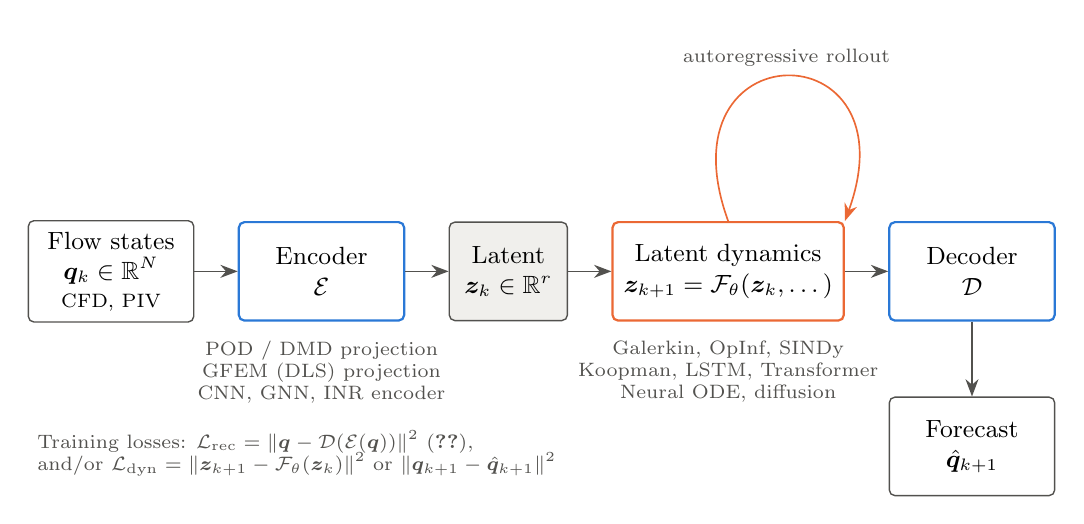
\begin{tikzpicture}[
    font=\small,
    box/.style={draw=cink2, line width=0.5pt, rounded corners=2pt, align=center,
                minimum height=1.25cm, inner sep=4pt, fill=white},
    lat/.style={box, fill=cneutral, minimum width=1.5cm},
    arr/.style={-{Stealth[length=2.2mm]}, line width=0.6pt, draw=cink2},
    note/.style={font=\scriptsize, text=cink2, align=center}
  ]
  \node[box, minimum width=2.1cm] (data) {Flow states\\$\q_k\in\R^{N}$\\[-1pt]{\scriptsize CFD, PIV}};
  \node[box, right=0.55cm of data, minimum width=2.1cm, draw=cblue, line width=0.8pt] (enc) {Encoder\\$\enc$};
  \node[lat, right=0.55cm of enc] (z) {Latent\\$\z_k\in\R^{r}$};
  \node[box, right=0.55cm of z, minimum width=2.4cm, draw=corange, line width=0.8pt] (dyn) {Latent dynamics\\$\z_{k+1}=\mathcal{F}_\theta(\z_{k},\dots)$};
  \node[box, right=0.55cm of dyn, minimum width=2.1cm, draw=cblue, line width=0.8pt] (dec) {Decoder\\$\dec$};
  \node[box, below=0.95cm of dec, minimum width=2.1cm] (out) {Forecast\\$\hat{\q}_{k+1}$};

  \draw[arr] (data) -- (enc);
  \draw[arr] (enc) -- (z);
  \draw[arr] (z) -- (dyn);
  \draw[arr] (dyn) -- (dec);
  \draw[arr] (dec) -- (out);
  \draw[arr, draw=corange] (dyn.north) to[out=110, in=70, looseness=4.5]
      node[note, above, pos=0.5] {autoregressive rollout} (dyn.north east);

  \node[note, below=0.12cm of enc] {POD / DMD projection\\GFEM (DLS) projection\\CNN, GNN, INR encoder};
  \node[note, below=0.12cm of dyn] {Galerkin, OpInf, SINDy\\Koopman, LSTM, Transformer\\Neural ODE, diffusion};

  \node[note, anchor=north west, align=left] at ($(data.south west)+(0,-1.25)$) {Training losses: $\mathcal{L}_{\mathrm{rec}}=\|\q-\dec(\enc(\q))\|^{2}$ (\cref{eq:generic}),\\ and/or $\mathcal{L}_{\mathrm{dyn}}=\|\z_{k+1}-\mathcal{F}_\theta(\z_k)\|^{2}$ or $\|\q_{k+1}-\hat{\q}_{k+1}\|^{2}$};
\end{tikzpicture}
\caption{Generic compress--evolve--reconstruct pipeline for data-driven modeling
of fluid flows. The encoder and decoder (blue) define the reduced
representation; the latent dynamics model (orange) is either derived by
projecting the governing equations (intrusive) or learned from encoded
trajectories (non-intrusive), and is iterated autoregressively at prediction
time. The two components can be trained sequentially (reconstruction loss,
then dynamics loss) or jointly.}
\label{fig:pipeline}
\end{figure}

\subsection{A taxonomy}

\Cref{fig:taxonomy} organizes the methods reviewed here along two axes: whether
the trial manifold is linear or nonlinear, and whether the representation is
global or spatially localized. Linear global bases (POD and its spectral
relatives, \cref{sec:linear}) remain the default. Sparse, clustered, and local
bases (\cref{sec:local}) keep linearity within a patch, cluster, or subdomain
but assemble a representation that is nonlinear or multi-scale overall.
Nonlinear manifold learning methods, both classical (\cref{sec:manifold}) and
neural (\cref{sec:autoencoders}), learn curved trial manifolds. Mesh-agnostic
and operator-based approaches (\cref{sec:meshfree}) relax the assumption of a
fixed discretization.

\begin{figure}[tbp]
\centering
\begin{forest}
  for tree={
    grow'=east, anchor=west, child anchor=west, parent anchor=east,
    draw=cink2, line width=0.4pt, rounded corners=1.5pt,
    font=\scriptsize, inner sep=2.5pt, l sep=4mm, s sep=1.0mm,
    edge={draw=cink2, line width=0.4pt},
    forked edges,
  },
  where level=0{font=\small\bfseries, align=center, fill=cneutral}{},
  where level=1{font=\footnotesize\bfseries, node options={text width=3.25cm, align=left}}{},
  where level=2{node options={text width=10.0cm, align=left}}{},
  [{DR for\\fluid ML}
    [{Linear subspace\\{\normalfont(\S\ref{sec:linear})}}, draw=cblue, line width=0.8pt
      [{POD/PCA, method of snapshots, randomized and streaming SVD}]
      [{DMD, Koopman/EDMD, SPOD, balanced POD, resolvent, mPOD}]
      [{Transport-adapted: shifted POD, registration, transported snapshots}]
    ]
    [{Sparse, clustered, local\\{\normalfont(\S\ref{sec:local})}}, draw=caqua, line width=0.8pt
      [{Sparse coding, dictionary learning, compressed sensing}]
      [{Clustered and local bases in state/parameter/time (local ROBs, cluster-based ROM)}]
      [{Spatial localization: RB element, DD-ROM, DD-LSPG, GFEM enrichment, DLS}]
    ]
    [{Classical manifold\\learning {\normalfont(\S\ref{sec:manifold})}}, draw=corange, line width=0.8pt
      [{Kernel PCA / kernel POD (pre-image problem)}]
      [{Isomap, LLE, Laplacian eigenmaps, diffusion maps; t-SNE, UMAP}]
      [{Polynomial and quadratic manifolds}]
    ]
    [{Neural autoencoders\\{\normalfont(\S\ref{sec:autoencoders})}}, draw=cviolet, line width=0.8pt
      [{MLP and convolutional AEs, mode-decomposing and hierarchical AEs}]
      [{VAE, $\beta$-VAE, VQ-VAE; rank-minimizing and dimension-discovering AEs}]
      [{Physics-constrained AEs, manifold Galerkin/LSPG}]
    ]
    [{Mesh-agnostic and\\operator {\normalfont(\S\ref{sec:meshfree})}}, draw=cmagenta, line width=0.8pt
      [{Graph autoencoders (multiscale, graph-convolutional)}]
      [{Implicit neural representations (NIF, CROM, DINo, CORAL, AROMA)}]
      [{Latent neural operators (PCA-Net, DeepONet, FNO, L-DeepONet, Transolver)}]
    ]
  ]
\end{forest}
\caption{Taxonomy of dimensionality reduction techniques used for machine learning
in fluid dynamics, with the section in which each family is reviewed.}
\label{fig:taxonomy}
\end{figure}

% ======================================================================
\section{Linear subspace methods}
\label{sec:linear}
% ======================================================================

\subsection{Proper orthogonal decomposition}
\label{sec:pod}

Proper orthogonal decomposition (POD), known in statistics as principal
component analysis (PCA) \parencite{pearson1901,hotelling1933} and in stochastic
processes as the Karhunen--Lo\`eve expansion, was introduced to turbulence by
\textcite{lumley1967} as an objective definition of coherent structures. Given
the snapshot matrix \eqref{eq:snapshots}, POD seeks the orthonormal basis
$\{\bm{\phi}_j\}_{j=1}^{r}$ that maximizes the average projected energy or,
equivalently, minimizes the mean-square reconstruction error
\begin{equation}
  \min_{\Phib^{\top}\W\Phib=\bm{I}}\;\sum_{k=1}^{T}\bigl\|\bm{x}_k-\Phib\Phib^{\top}\W\bm{x}_k\bigr\|_{\W}^{2},
  \label{eq:pod}
\end{equation}
whose solution is given by the leading left singular vectors of
$\W^{1/2}\X$. With the singular value decomposition
$\W^{1/2}\X=\bm{U}\bm{\Sigma}\bm{V}^{\top}$, the modes are
$\Phib=\W^{-1/2}\bm{U}_{:,1:r}$, the temporal coefficients are
$\z_k=\Phib^{\top}\W\bm{x}_k$, and the eigenvalues $\lambda_j=\sigma_j^2$ are the
energies of the modes. By the Eckart--Young theorem \parencite{eckart1936},
the truncation error is $\sum_{j>r}\lambda_j$, so no rank-$r$ linear
representation of the \emph{training} data is more accurate in this norm. When
$T\ll N$, as is typical for simulation data, the \emph{method of snapshots}
\parencite{sirovich1987} obtains the same modes from the $T\times T$
correlation matrix $\X^{\top}\W\X$. The theory and early applications to wall
turbulence and transitional flows are reviewed by \textcite{berkooz1993} and
\textcite{holmes2012turbulence}.

POD has several properties that explain its dominance as the first stage of
fluid-dynamics ML pipelines. Its encoder and decoder are linear, cheap, and
exactly inverse on the subspace. The modes are orthogonal and ranked by
energy. For many flows the leading modes have clear physical meaning, for
example the pairs of traveling-wave modes associated with vortex shedding. The
construction requires no hyperparameters beyond $r$. Scalable algorithms are
mature: randomized SVD \parencite{halko2011} and incremental or streaming SVD
\parencite{levy2000,brand2006} make POD feasible for data sets that do not fit
in memory.

\Cref{fig:ldc_pod} shows POD applied to a two-dimensional lid-driven cavity at
$\mathrm{Re}=15{,}000$, the dataset used for the computed examples in this
review. The leading modes are organized along the shear layers and walls of the
cavity. The first two modes form a traveling-wave pair that together capture
about 90\% of the fluctuation energy, and eight modes capture 99\%. A spectrum
this steep indicates a flow dominated by a small number of coherent
oscillations, the regime in which global POD is most effective. We return to
this point when comparing global and local bases in \cref{sec:dls}.

\begin{figure}[tbp]
  \centering
  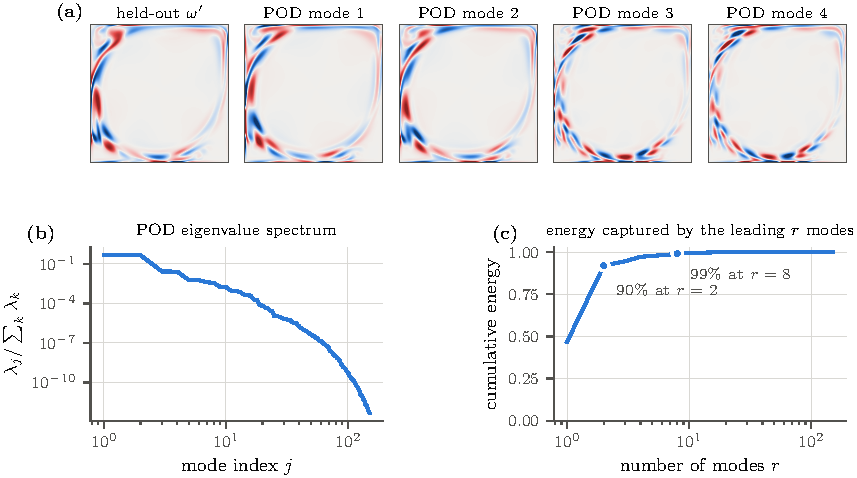
\includegraphics[width=\textwidth]{figs/ldc_pod.pdf}
  \caption{POD of the two-dimensional lid-driven cavity at $\mathrm{Re}=15{,}000$
  (2000 training snapshots, weighted $L^2$ inner product). (a)~Fluctuating
  vorticity of a held-out snapshot and of the four leading POD modes;
  (b)~normalized eigenvalue spectrum (modes with $\lambda_j>10^{-12}\lambda_1$);
  (c)~cumulative energy fraction, with the number of modes needed to capture
  90\% and 99\% of the fluctuation energy.}
  \label{fig:ldc_pod}
\end{figure}

\paragraph{POD in intrusive models.}
The classical use of POD is Galerkin projection of the Navier--Stokes equations
onto the leading modes. Early landmarks include the low-dimensional model of
the turbulent wall layer of \textcite{aubry1988}, and the hierarchy of cylinder
wake models of \textcite{noack2003hierarchy}, which introduced a ``shift mode''
to represent the mean-flow deformation that POD modes of the limit cycle
miss. Two difficulties of POD--Galerkin models motivate much of the later
data-driven work. First, truncation removes the small scales that dissipate
energy, so truncated models are often unstable or inaccurate without closure
\parencite{wang2012closure,ahmed2021closures}. Second, evaluating the nonlinear
term still scales with $N$ unless hyper-reduction is used, for example the
empirical and discrete empirical interpolation methods
\parencite{barrault2004eim,chaturantabut2010deim} or GNAT with least-squares
Petrov--Galerkin (LSPG) projection
\parencite{carlberg2011lspg,carlberg2013gnat,carlberg2017galerkin}.

\paragraph{POD in non-intrusive, learned models.}
Because POD coefficients form a compact, ordered, and decorrelated set of
features, they are the most common input to learned surrogate models. In
parametric problems, regression maps from parameters (and time) to POD
coefficients have been built with neural networks
\parencite{hesthaven2018podnn} and Gaussian processes \parencite{guo2019gpr}.
PCA-Net extends the idea to operator learning by applying PCA to both input and
output function spaces \parencite{bhattacharya2021pcanet}. For time-series
prediction, POD coefficients have been advanced by extreme learning machines
used as closures \parencite{san2018elm} and by recurrent networks:
long short-term memory (LSTM) models of POD coefficients were proposed by
\textcite{wang2018model} and by \textcite{mohan2018lstm} for turbulent-flow
control, deep feedforward networks with residual and backward-difference update
formulas by \textcite{pawar2019deep}, and LSTMs and neural ordinary differential
equations, including closure of unresolved modes, by
\textcite{maulik2020timeseries}. More recently, transformers have been applied
to POD coefficients of flows past a cylinder and a group of buildings
\parencite{wu2022transformer}. Operator inference fits polynomial reduced
operators directly to projected trajectories
\parencite{peherstorfer2016opinf,qian2020liftlearn,kramer2024opinf}; it is
non-intrusive but, unlike black-box regression, retains the structure of a
projection-based ROM. \textcite{swischuk2019projection} compare several such
POD-plus-regression formulations and argue that the projection structure is
itself a useful physics-based inductive bias.

\subsection{Dynamics- and frequency-aware decompositions}
\label{sec:dmd}

POD ranks modes by energy but ignores temporal order. Several decompositions
incorporate dynamics or frequency content and are frequently used either as
the reduced representation or as a diagnostic of it.

\emph{Dynamic mode decomposition} (DMD) fits a best linear operator
$\bm{A}$ with $\bm{x}_{k+1}\approx\bm{A}\bm{x}_k$ and represents the data by
its eigenvectors, each oscillating at a single frequency with a single growth
rate \parencite{schmid2010dmd}. \textcite{rowley2009spectral} interpreted DMD
as a finite-dimensional approximation of the Koopman operator
\parencite{mezic2005,mezic2013}. Exact DMD \parencite{tu2014dmd}, extended DMD
with nonlinear dictionaries \parencite{williams2015edmd}, sparsity-promoting DMD
\parencite{jovanovic2014spdmd}, and optimized DMD \parencite{askham2018optdmd}
are variants that improve robustness or mode selection; see
\textcite{kutz2016dmd} and \textcite{brunton2022koopman} for reviews. For
learning, the appeal of DMD and Koopman methods is that they provide
coordinates in which the dynamics are (approximately) linear, an idea that
reappears in Koopman autoencoders (\cref{sec:koopman}).

\emph{Spectral POD} (SPOD) computes POD modes of each temporal frequency from
the cross-spectral density, yielding modes that are coherent in both space and
time and optimal for statistically stationary flows
\parencite{towne2018spod,schmidt2020guide}. Towne et al.\ showed that SPOD modes
coincide with DMD modes and with resolvent modes
\parencite{mckeon2010critical} under particular assumptions. A distinct method
with the same name filters the POD correlation matrix along its diagonals to
interpolate between POD and a Fourier decomposition \parencite{sieber2016spod}.
\emph{Multi-scale POD} (mPOD) combines a filter bank with POD so that each
mode is confined to a frequency band \parencite{mendez2019mpod}, which is
relevant for flows with several separated time scales.
\emph{Balanced POD} \parencite{rowley2005bpod} approximates balanced truncation
\parencite{moore1981} using snapshots of the direct and adjoint systems, and
selects modes by input--output importance rather than energy. This matters
for control-oriented models, where low-energy structures can dominate the
response.

\subsection{Limits of global linear reduction}
\label{sec:barrier}

The optimality of POD is optimality \emph{among linear subspaces for the
training data}. Two limitations follow.

\paragraph{The transport barrier.}
When coherent features move, such as a vortex advected through the domain, a
shock translating with a parameter, or a flame front, the set of states is a
low-dimensional but strongly curved manifold whose linear span is large. For
the linear advection equation with discontinuous data, the Kolmogorov $n$-width
\eqref{eq:nwidth} decays only as $r^{-1/2}$
\parencite{ohlberger2016reduced,greif2019decay}. \Cref{fig:nwidth} shows the
effect on the singular values of simple one-dimensional snapshot sets. For a
diffusing Gaussian pulse the singular values fall below $10^{-10}$ within
about twenty modes. For the same pulse advected across the domain they decay
far more slowly. For an advected discontinuity they remain above $10^{-2}$ for
more than a hundred modes, until the snapshot matrix runs out of rank. Such
problems are common in fluid dynamics: shear layers, wakes, jets, cavity
flows with convecting vortices, and shocks all feature transport.

Within the linear framework, the barrier can be mitigated by transforming the
data before POD so that the features no longer move. Approaches include
symmetry reduction and template fitting \parencite{rowley2000symmetry},
Lagrangian or characteristic-based bases \parencite{mojgani2017lagrangian},
shifted POD with multiple transport velocities \parencite{reiss2018spod},
optimal-transport advection modes \parencite{iollo2014advection},
transport reversal \parencite{rim2018transport}, transported snapshots
\parencite{nair2019transported}, and learned registration maps
\parencite{taddei2020registration,mojgani2021registration}. All of these build
a \emph{nonlinear} trial manifold out of a linear basis and a nonlinear
transformation, and they anticipate the neural approaches of
\cref{sec:autoencoders}. \textcite{peherstorfer2022breaking} provides a concise
review of this line of work.

\paragraph{Multi-scale content and generalization.}
High-Reynolds-number turbulence poses a related difficulty even without a
dominant transport direction. The energy spectrum is broadband, so the POD
eigenvalues decay slowly and the small scales, which carry a small share of the
energy but most of the dissipation and much of the intermittency, sit at the
end of the spectrum. The global modes also have global support: a mode that
represents a structure in one region must also be ``paid for'' everywhere
else. In addition, the rank of a snapshot POD basis cannot exceed the number
of training snapshots, so for flows with many active scales the amount of
training data needed grows with the desired accuracy. It is well documented
that POD bases can be inefficient for multi-scale turbulent flows
\parencite{berkooz1993,deshmukh2016sparse,deshmukh2020dls}. Parametric variation
adds a third difficulty: a basis built at one operating condition may not
represent another. Common remedies are interpolation of bases on the
Grassmann manifold \parencite{amsallem2008grassmann} and the local and
clustered bases discussed next.

\begin{figure}[tbp]
  \centering
  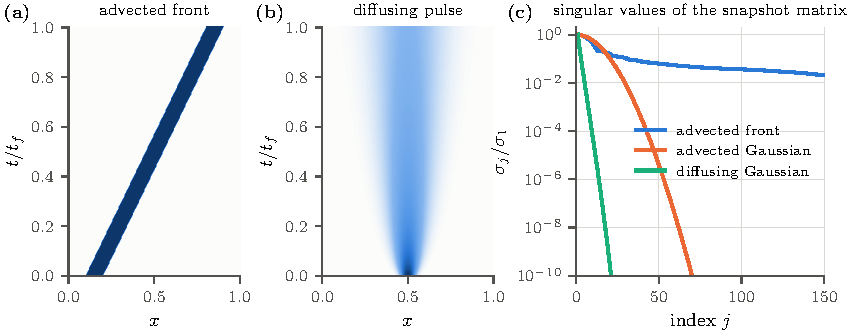
\includegraphics[width=\textwidth]{figs/nwidth.pdf}
  \caption{The transport barrier for linear reduction. (a)~An advected
  discontinuity (top-hat of width 0.1) and (b)~a diffusing Gaussian pulse,
  shown in space--time. (c)~Normalized singular values of the corresponding
  snapshot matrices (200 snapshots, 256 grid points), together with an
  advected Gaussian of the same width as the diffusing pulse. All three
  data sets are one-parameter families, yet for a given accuracy the advected
  families need several times (Gaussian) to tens of times (discontinuity) more
  linear modes than the diffusing one.}
  \label{fig:nwidth}
\end{figure}

% ======================================================================
\section{Sparse, clustered, and spatially localized representations}
\label{sec:local}
% ======================================================================

A global linear basis must represent every state as a superposition of the
same $r$ modes, each supported on the whole domain. The methods in this section
relax one of these two features. Sparse and clustered representations let the
set of active modes depend on the state. Spatially localized representations
restrict the support of each basis function to a subdomain. The resulting
representations are piecewise linear in state space or in physical space, and
therefore nonlinear or multi-scale overall. They keep much of the transparency,
cost, and robustness of linear methods.

\subsection{Sparse coding and dictionary learning}

Sparse coding represents each state as a combination of a few atoms from an
overcomplete dictionary $\bm{D}\in\R^{N\times K}$ with $K>N$ or $K>r$,
\begin{equation}
  \min_{\bm{D},\{\bm{s}_k\}}\;\sum_{k}\|\bm{x}_k-\bm{D}\bm{s}_k\|_2^2+\lambda\|\bm{s}_k\|_1,
\end{equation}
so that different states can activate different subsets of atoms.
Dictionaries learned from natural images reproduce the localized, oriented
receptive fields of the visual cortex \parencite{olshausen1996}. K-SVD is a
widely used algorithm for learning them \parencite{aharon2006ksvd}.
\textcite{deshmukh2016sparse} introduced sparse coding for basis identification
in fluid ROMs. Unlike POD, which truncates to the dominant energetic modes,
sparse coding seeks a compact representation spanning \emph{all} scales of the
data, and Galerkin models built on sparse modes of a lid-driven cavity flow were
substantially more predictive than POD--Galerkin models.
\textcite{deshmukh2018energy} traced this improvement to energy balance.
Multi-scale content in the retained modes lets the ROM balance production and
dissipation of energy, which a basis made only of large, energetic structures
cannot. Sparsity is also the foundation of compressed sensing
\parencite{candes2006robust,donoho2006cs}, which in fluids underlies sparse
sensor placement \parencite{manohar2018sensor} and flow reconstruction by
sparse representation in a library of training snapshots
\parencite{callaham2019robust}.

\subsection{Clustered and local bases in state, parameter, and time}

A second way to adapt the representation to the state is to partition the data
set and assign a separate low-dimensional description to each part.
\emph{Cluster-based reduced-order modeling} \parencite{kaiser2014cluster}
partitions snapshots into a small number of clusters by $k$-means, represents
each by its centroid, and models the dynamics as a Markov chain of transitions
between clusters, generalizing the Ulam--Galerkin approximation of the
Perron--Frobenius operator. \emph{Local reduced-order bases}
\parencite{amsallem2012local} cluster the solution space and build a separate
POD basis for each cluster, switching bases online as the state moves between
regions. They are aimed at problems with distinct physical regimes, parameter
variations, or moving fronts. Related ideas include local discrete empirical
interpolation \parencite{peherstorfer2014ldeim} and interpolation of bases
between parameter values on the Grassmann manifold
\parencite{amsallem2008grassmann}. These methods approximate a curved manifold
by a patchwork of tangent-like subspaces, a strategy mirrored in locally linear
embedding (\cref{sec:manifold}) and in the local linear decoder used by
\textcite{loiseau2018sparse}.

\subsection{Spatial localization and domain decomposition}

Localization in \emph{physical} space follows from a simple observation.
Correlations in turbulent flows decay with separation, so a structure in one
region carries little information about another. A global mode that captures a
structure in one region wastes degrees of freedom elsewhere, whereas a local
basis spends them only where needed and can be reused wherever similar
structures appear. Wavelet decompositions, which are localized in both
space and scale, were an early expression of this idea in turbulence analysis
\parencite{farge1992wavelet}. The idea has a long history in both reduced-order
modeling and numerical analysis.

In reduced-order modeling, \textcite{lucia2001thesis,lucia2003moving} treated the region swept by
a moving shock separately from the rest of a POD-based model, isolating the
feature that a global basis represents worst. The reduced basis element method
\parencite{maday2002rbe} and the static-condensation reduced basis element
method \parencite{huynh2013scrbe} build reduced bases for components or
subdomains and couple them across interfaces. Domain-decomposition strategies
have been developed for POD-based models of the incompressible Navier--Stokes
equations \parencite{baiges2013dd} and for reduced-basis methods in networks
and complex geometries \parencite{iapichino2016dd}. For extreme-scale problems,
where even storing global snapshots is prohibitive, domain-decomposition
least-squares Petrov--Galerkin (DD-LSPG) builds subdomain bases and couples
them through the governing equations \parencite{hoang2021ddlspg}.
\textcite{diaz2024ddnm} extended this approach to nonlinear manifolds, training
a separate shallow sparse autoencoder on each subdomain. The subdomain models
have fewer parameters, need smaller training sets, and can be trained in
parallel.

In numerical analysis, the partition-of-unity finite element method
\parencite{melenk1996pum} and the generalized finite element method (GFEM)
\parencite{babuska2004gfem} showed how to embed arbitrary local approximation
spaces into a conforming global approximation. Let $\{N_i\}$ be finite element
shape functions forming a partition of unity, $\sum_i N_i\equiv 1$, each
supported on the patch $\omega_i$ of elements sharing node $i$. Let
$\{\psi_{i,k}\}$ be any functions that approximate the solution well on
$\omega_i$. Then
\begin{equation}
  u(\bm{x})\approx\sum_{i}N_i(\bm{x})\Bigl[a_i+\sum_{k=1}^{m}b_{ik}\,\psi_{i,k}(\bm{x})\Bigr]
  \label{eq:gfem}
\end{equation}
inherits the local approximation quality of the enrichments $\psi_{i,k}$, while
the multiplication by $N_i$ keeps every basis function compactly supported and,
for continuous $N_i$ and $\psi_{i,k}$, globally $C^{0}$
\parencite{melenk1996pum}. \textcite{babuska2011optimal} characterized optimal
local approximation spaces for GFEM in multi-scale problems;
\textcite{smetana2016optimal} did the same for component-based static
condensation. The multiscale finite element method
\parencite{hou1997msfem} and its generalized variant
\parencite{efendiev2013gmsfem} construct local basis functions from local
solutions or local snapshot spaces. This is the same idea of numerically
computed, locally supported bases, derived from the operator instead of from
data.

\subsection{Data-informed local subspaces}
\label{sec:dls}

The Data-informed Local Subspace (DLS) method of \textcite{deshmukh2020dls}
brings the GFEM construction \eqref{eq:gfem} to data-driven representation of
turbulent flows. The enrichment functions are learned from snapshot data rather
than derived from the governing operator. The construction has four steps,
illustrated in one dimension in \cref{fig:dls_schematic}.
\begin{enumerate}[leftmargin=2.2em,itemsep=2pt]
  \item \emph{Coarse mesh and partition of unity.} A coarse mesh of linear (in
  two dimensions, bilinear) finite elements is laid over the data grid with
  nodes every $n_{\mathrm{skip}}$ grid points; its shape functions $N_i$ form
  a partition of unity (\cref{fig:dls_schematic}a).
  \item \emph{Local POD modes.} Patches of $(2n_{\mathrm{skip}}+1)^{d}$ grid
  points are sampled at random locations from the training snapshot(s). The
  mean of each patch is removed, and the patches are decomposed by POD
  (\cref{fig:dls_schematic}b). The leading $m$ local modes $\psi_k$ are shared
  by all nodes: the mode used at node $i$ is $\psi_k(\bm{x}-\bm{x}_i)$,
  centered on the node, so that its $(2n_{\mathrm{skip}}+1)^{d}$ footprint
  exactly covers the support $\omega_i$ of $N_i$.
  \item \emph{GFEM enrichment.} The local modes are multiplied by the shape
  functions, and the products $N_i(\bm{x})\,\psi_k(\bm{x}-\bm{x}_i)$ are used,
  together with the standard $N_i$, as the basis functions of \eqref{eq:gfem}
  (\cref{fig:dls_schematic}c). Each enrichment vanishes on the boundary of
  $\omega_i$, so the assembled representation is $C^{0}$-continuous across
  element boundaries. The local POD modes are thus not used directly as a
  block-wise basis: they enter only through the enriched GFEM space.
  \item \emph{Global projection.} The $(m+1)$ coefficients per node and field
  variable are obtained by $L^2$ projection onto the enriched space. The global
  mass matrix $\bm{M}$ is assembled from element matrices, and the load vector
  $\bm{L}$ from element-wise inner products with the data, giving
  $\bm{M}\bm{c}=\bm{L}$. On a uniform mesh with shared local modes all
  element mass matrices are identical, so $\bm{M}$ is sparse and is factorized
  once (\cref{fig:dls_schematic}d).
\end{enumerate}
The latent vector $\bm{c}$ has dimension $r=d_v\,n_{\mathrm{nodes}}\,(m+1)$
for $d_v$ field variables. Only the $m$ local modes of size
$(2n_{\mathrm{skip}}+1)^{d}$ per variable need to be stored in addition to the
coefficients. Following \textcite{deshmukh2020dls}, the compression ratio for
$T$ snapshots of an $M$-dimensional field in $d$ spatial dimensions (with $d$
velocity components) is
\begin{equation}
  \mathrm{CR}=\frac{M\,T}{d\,T\,n_{\mathrm{nodes}}(m+1)+d\,m\,(2n_{\mathrm{skip}}+1)^{d}}.
\end{equation}
Encoder and decoder are both linear, sparse, and local. The encoder is a
sparse linear solve and the decoder an element-wise sum.

Several properties make DLS attractive as a representation for learning.
(i) \emph{Data efficiency (P4).} Because patches are sampled \emph{within}
snapshots, a single snapshot provides thousands of training samples for the
local modes. \textcite{deshmukh2020dls} reported that, relative to global POD,
the GFEM approach increases reconstruction efficiency for a three-dimensional
cylinder flow at $\mathrm{Re}=10^{5}$ and for lid-driven cavity flows over a
range of Reynolds numbers, while substantially reducing the amount of training
data required. (ii) \emph{Multi-scale resolution (P1).} The coarse element size
sets the scale resolved by the standard FE part, and the local modes add
sub-element structure, so resolution is controlled locally rather than by
global energy ranking. (iii) \emph{Scalability (P5).} Encoding and decoding
are sparse operations whose cost grows linearly with $N$, and the basis is
independent of the number of snapshots. (iv) \emph{Structured latent space.}
The coefficients are attached to mesh nodes, so the latent state is itself a
coarse spatial field. Sequence models can therefore operate on it globally or
as spatially local tokens, analogous to the patch tokens of vision transformers
\parencite{dosovitskiy2021vit} or the local neural fields of AROMA
\parencite{serrano2024aroma}. The price is a larger latent dimension than a
global basis needs when the flow is dominated by a few coherent structures.

\textcite{morton2026scitech} used DLS latent spaces with transformer forecasting
for two-dimensional lid-driven cavity flow at $\mathrm{Re}=15{,}000$ and
$30{,}000$. They found that the DLS-based model reasonably reproduced the flow
dynamics and turbulence statistics at both Reynolds numbers, whereas models
trained on a POD latent space performed poorly. A related precedent for
exploiting locality in the \emph{dynamics} model is the parallel reservoir
computing approach of \textcite{pathak2018reservoir}, in which many small
reservoirs each forecast a local region of a large spatiotemporally chaotic
system.

\paragraph{A computed comparison.}
\Cref{fig:dls_compare,fig:dls_recon} compare global POD and DLS on held-out
snapshots of the $\mathrm{Re}=15{,}000$ cavity flow of \cref{fig:ldc_pod}.
DLS bases use local modes from a single training snapshot, while the POD basis
uses 2000 snapshots. Three observations follow. First,
at equal latent dimension global POD is far more compact for this flow
(\cref{fig:dls_compare}a). Its held-out error falls to 0.33\% with about 150
modes, beyond which the remaining modes carry negligible energy. DLS needs
roughly $10^{4}$ coefficients for 1\% error ($49^2$ patches, $m=10$) and
$2.6\times10^{4}$ for 0.45\% ($19^2$, $m=3$). At a budget of 1936
coefficients, DLS errors are 11--13\%, and the vorticity reconstructions show
element-scale artifacts (\cref{fig:dls_recon}). This is the expected outcome
for a flow whose fluctuation energy is 90\% contained in a single pair of
global modes (\cref{fig:ldc_pod}). Second, the comparison reverses when the
amount of training data is considered (\cref{fig:dls_compare}b). A POD basis
built from the first 512 snapshots has a held-out error of 8.3\%, and one
built from 1000 snapshots 1.8\%, whereas DLS bases whose local modes come from
a \emph{single} snapshot reach 1.0\% ($49^2$, $m=10$) and 0.45\% ($19^2$,
$m=3$). DLS accuracy is set by local resolution ($n_{\mathrm{skip}}$ and $m$),
not by how much of the flow's temporal variability the training record
happens to contain. Third, the singular values of small local patches decay
faster than those of the global snapshots (\cref{fig:dls_compare}c), which is
the local redundancy that the enrichment exploits. The example thus
illustrates the trade-off discussed in \cref{sec:assessment}. Global bases are
most compact for globally simple flows once enough data are available. Local
bases are data-efficient and scale with local rather than global complexity,
which matters most for broadband, multi-scale flows and for large domains
where long training records are unaffordable. Compactness of reconstruction
is also not the same as suitability for forecasting (\cref{sec:goodlatent}):
for this same cavity flow, \textcite{morton2026scitech} found transformer
forecasts on DLS latent spaces to be markedly better than on a POD latent
space.

\begin{figure}[tbp]
  \centering
  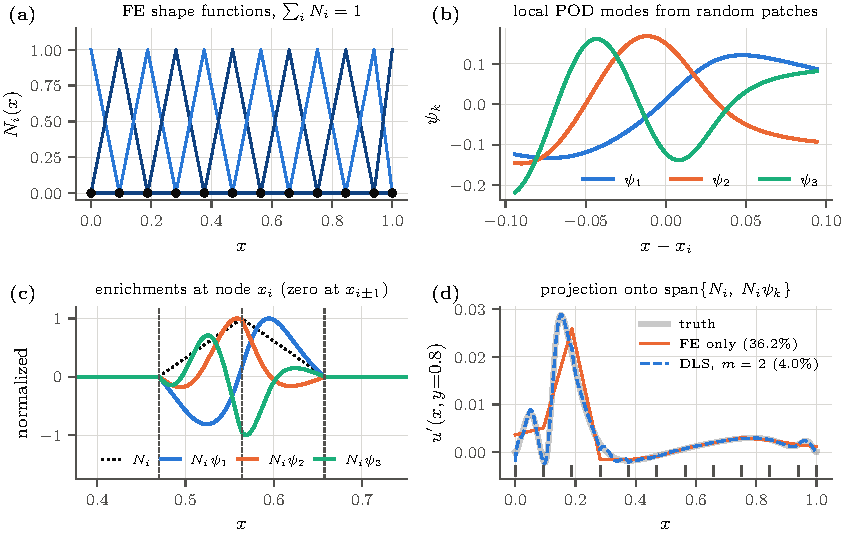
\includegraphics[width=\textwidth]{figs/dls_schematic.pdf}
  \caption{The DLS/GFEM construction in one dimension, applied to a horizontal
  line cut ($y=0.8$) of the fluctuating velocity in the $\mathrm{Re}=15{,}000$
  cavity. (a)~Linear finite element shape functions on a coarse mesh (nodes
  every $n_{\mathrm{skip}}=48$ grid points) form a partition of unity.
  (b)~Leading local POD modes of randomly sampled, mean-removed patches of
  $2n_{\mathrm{skip}}+1$ points. (c)~Enrichment functions
  $N_i(x)\,\psi_k(x-x_i)$ at one node: each is supported on the two elements
  adjacent to $x_i$ and vanishes at $x_{i\pm1}$, which guarantees
  $C^{0}$ continuity of the assembled field. (d)~$L^2$ projection of the signal
  onto the standard FE space alone and onto the enriched space with $m=2$ local
  modes; relative errors in parentheses.}
  \label{fig:dls_schematic}
\end{figure}


\begin{figure}[tbp]
  \centering
  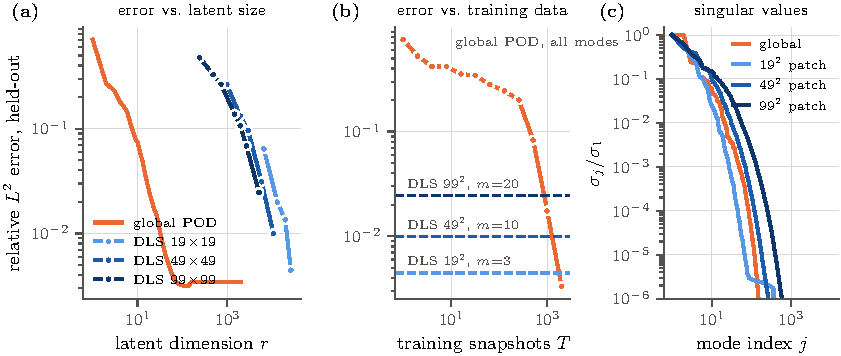
\includegraphics[width=\textwidth]{figs/ldc_local_global.pdf}
  \caption{Global POD versus DLS for the $\mathrm{Re}=15{,}000$ lid-driven cavity.
  (a)~Relative $L^2$ error of the fluctuating velocity on 90 held-out snapshots
  (separated in time from the training window) versus latent dimension. POD
  uses 2000 training snapshots; DLS uses local modes from a single training
  snapshot, with patch sizes $19^2$, $49^2$, and $99^2$ and
  $m$ local modes per node (markers, increasing $m$ from left).
  (b)~Error of global POD, keeping all non-negligible modes, when built from
  the first $T$ training snapshots. Dashed lines give the DLS errors of
  panel~(a) for the largest $m$ of each patch size, obtained from one snapshot.
  (c)~Normalized singular values of the global snapshot matrix and of the
  random local patches used to build the DLS modes. Errors are evaluated on
  the $491\times491$ region covered by all DLS meshes.}
  \label{fig:dls_compare}
\end{figure}

\begin{figure}[tbp]
  \centering
  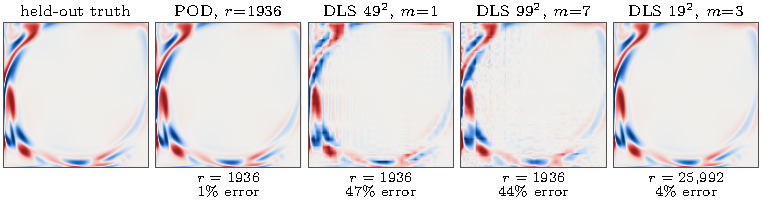
\includegraphics[width=\textwidth]{figs/ldc_local_recon.pdf}
  \caption{Fluctuating vorticity of a held-out cavity snapshot and its
  reconstructions. The middle three panels use the same number of latent
  coefficients ($r=1936$; for POD this includes all $\approx150$ modes with
  non-negligible energy). The right panel shows DLS with $19^2$ patches and
  $m=3$ ($r=25{,}992$). Percentages are relative $L^2$ errors of the
  vorticity, which weights small scales more heavily than the velocity errors
  of \cref{fig:dls_compare}.}
  \label{fig:dls_recon}
\end{figure}

% ======================================================================
\section{Classical nonlinear manifold learning}
\label{sec:manifold}
% ======================================================================

Before neural autoencoders became practical, a family of nonlinear DR methods
was developed in machine learning to recover low-dimensional coordinates for
data lying near curved manifolds. These methods work directly with the data
set, often through a similarity graph or kernel matrix, and learn an
\emph{embedding} of the training points. Most do not provide a decoder, which
has limited their use as reduced representations for dynamics but made them
valuable for analysis and for estimating intrinsic dimension.

\subsection{Kernel principal component analysis}

Kernel PCA \parencite{scholkopf1998kpca} performs PCA in a feature space defined
implicitly by a positive-definite kernel $k(\bm{x},\bm{x}')$, for example a
Gaussian or polynomial kernel. The embedding coordinates follow from the
eigenvectors $\bm{\alpha}_j$ of the centered $T\times T$ kernel matrix,
$z_j(\bm{x})=\sum_{i}\alpha_{j,i}\,k(\bm{x}_i,\bm{x})$, so kernel PCA is the
nonlinear analogue of the method of snapshots and has the same cost scaling.
Reconstruction requires solving a \emph{pre-image} problem, finding a state
whose feature-space image is close to a given point, which is ill-posed and
usually solved approximately by fixed-point iteration or regression
\parencite{mika1999preimage}. \textcite{salvador2021kpod} used kernel POD to
build reduced spaces for parametrized PDEs and trained neural networks to
predict the reduced coefficients. They obtained more accurate snapshot
approximations with fewer coordinates than POD at similar online cost.

\subsection{Graph-based spectral embeddings}

Isomap \parencite{tenenbaum2000isomap} approximates geodesic distances on the
manifold by shortest paths in a nearest-neighbour graph and embeds them with
multidimensional scaling. Locally linear embedding (LLE)
\parencite{roweis2000lle} computes weights that reconstruct each point from its
neighbours and finds low-dimensional coordinates that preserve those weights.
Laplacian eigenmaps \parencite{belkin2003laplacian} and diffusion maps
\parencite{coifman2006diffusion} use eigenvectors of a graph Laplacian or of a
Markov diffusion operator on the data. Diffusion maps add a time parameter
that exposes the geometry at multiple scales. All of these methods preserve
local neighbourhoods and can unfold manifolds that linear projections fold
onto themselves.

In fluid dynamics, \textcite{farzamnik2023snapshots} combined Isomap as an
encoder with a $k$-nearest-neighbour decoder. For the fluidic pinball they
described both the pitchfork bifurcation and the chaotic regime with only
three coordinates, linked to vortex-shedding phases and force coefficients.
For the wake of tandem cylinders, Isomap separated two shedding regimes that
appear as a single circle in the plane of the first two POD amplitudes.
\textcite{csala2022comparing} compared four manifold-learning and two
autoencoder methods with PCA on canonical laminar and turbulent flows and on
biomedical flows. They discussed the influence of arranging data temporally
versus spatially and concluded that nonlinear DR is promising for reduced-order
modeling. \textcite{mendez2023linear} placed kernel PCA, Isomap, and LLE in a
common framework with autoencoders and benchmarked them for filtering,
identification of oscillatory patterns, and compression.
\textcite{loiseau2018sparse} lifted sensor signals to a feature space by time
delays, identified sparse dynamics on it, and reconstructed the velocity field
with a local linear map from features to flow. This is another way to supply
the decoder that spectral embeddings lack.

The limitations of these methods for reduced-order modeling are well
recognized \parencite{mojgani2021registration}. There is no explicit map from
latent coordinates back to the physical space, and out-of-sample points need
Nystr\"om-type extensions. The embeddings depend on neighbourhood parameters,
and the coordinates are often hard to interpret. Cost and memory scale with
$T^{2}$. Visualization methods such as t-SNE \parencite{vandermaaten2008tsne}
and UMAP \parencite{mcinnes2018umap} are useful for exploring the structure of
flow data sets, but they deliberately distort global geometry and are not
suitable as coordinates for dynamics models. Manifold-learning estimates of
intrinsic dimension, such as the maximum-likelihood estimator of
\textcite{levina2004intrinsic}, remain useful for choosing latent sizes of the
autoencoders discussed next.

\subsection{Polynomial and quadratic manifolds}

A simple way to curve a linear subspace while keeping an explicit decoder is
to add polynomial corrections,
\begin{equation}
  \q\approx\bar{\q}+\bm{V}\z+\bm{H}\,(\z\otimes\z),
  \label{eq:quadratic}
\end{equation}
where $\bm{V}$ is usually a POD basis and $\bm{H}$ is fitted to the residual.
Quadratic manifolds were introduced for nonlinear structural dynamics
\parencite{jain2017quadratic}. They were later developed to mitigate the
Kolmogorov barrier in projection-based model reduction
\parencite{barnett2022quadratic} and combined with operator inference for
non-intrusive models \parencite{geelen2023quadratic}. The decoder
\eqref{eq:quadratic} is cheap and differentiable, the encoder can remain a
linear projection, and the construction is a small step from standard POD
workflows. The expressiveness is limited compared with deep networks, but
quadratic manifolds provide a useful intermediate baseline between linear and
fully learned trial manifolds.

% ======================================================================
\section{Neural-network autoencoders}
\label{sec:autoencoders}
% ======================================================================

\subsection{From nonlinear PCA to deep autoencoders}

An autoencoder (AE) parametrizes the encoder and decoder of \eqref{eq:generic}
with neural networks, $\z=\enc_{\theta}(\q)$ and $\hat{\q}=\dec_{\vartheta}(\z)$,
and trains both jointly to minimize reconstruction error through a bottleneck
of width $r$. \textcite{kramer1991nlpca} introduced this ``autoassociative''
architecture as nonlinear PCA. \textcite{baldi1989} had shown that a
\emph{linear} autoencoder trained with a squared loss has no spurious local
minima and that its optimum spans the principal subspace. A linear AE therefore
recovers the POD subspace, though not the ordered, orthogonal modes.
\textcite{hinton2006reducing} demonstrated that deep AEs can substantially
outperform PCA on image data. In fluid dynamics, \textcite{milano2002}
reproduced the POD equivalence for near-wall turbulence and showed that
nonlinear networks improved reconstruction and prediction of the near-wall
velocity field at small additional cost, a result that anticipated much of the
later literature.

\subsection{Convolutional autoencoders and nonlinear-manifold ROMs}

Fully connected AEs scale poorly with the number of grid points. Convolutional
AEs (CAEs) exploit spatial locality, weight sharing, and hierarchical
downsampling, which makes them the dominant architecture for gridded flow data.
\textcite{lee2020cae} showed that a deep CAE defines a nonlinear trial manifold
onto which the governing equations can be projected by manifold Galerkin or
manifold LSPG, with the decoder Jacobian replacing the basis matrix. The
resulting intrusive ROMs outperformed even the optimal linear subspace on
advection-dominated problems. Non-intrusive counterparts learn the latent
dynamics as well. \textcite{gonzalez2018deep} proposed convolutional recurrent
autoencoders. The DL-ROM of \textcite{fresca2021dlrom} learns both the trial
manifold and the reduced dynamics with a CAE and a feedforward network, and
POD-DL-ROM \parencite{fresca2022poddlrom} first applies POD (randomized SVD)
and trains the AE on POD coefficients, which cuts training cost substantially
at little loss of accuracy. Nonlinear-manifold ROMs have also been made fast
enough for practical use with hyper-reduction, through shallow, sparsely
connected (masked) decoders \parencite{kim2022shallow} and reduced
over-collocation \parencite{romor2023overcollocation}.

For unsteady flows, the most common pattern couples a CAE with a recurrent
network trained afterwards on the latent sequence. \textcite{omata2019} used a
CAE to obtain low-dimensional representations of unsteady flow fields that
preserve spatial structure. \textcite{eivazi2020deep} combined an AE with an
LSTM and compared it with POD-based alternatives.
\textcite{hasegawa2020bluff} trained CNN-AE/LSTM models on flows around 80
randomly shaped bluff bodies and tested them on 20 unseen shapes, and
\textcite{nakamura2021channel} extended the approach to three-dimensional
minimal turbulent channel flow at $\mathrm{Re}_{\tau}=110$.
\textcite{maulik2021advection} showed that a two-dimensional CAE latent space
suffices to reproduce a sharp advecting shock of the viscous Burgers equation,
and a six-dimensional one the inviscid shallow-water equations. They concluded
that such advection-dominated systems are more amenable to CAE--RNN models than
to POD--Galerkin models.
\textcite{xu2020multilevel} nested a spatial CAE, a temporal convolutional AE,
and a multilayer perceptron for parametric prediction of spatio-temporal
dynamics. \textcite{racca2023caesn} paired a CAE with an echo state network to
forecast turbulent dynamics.

A parallel line of work uses AEs to interpret flows. The mode-decomposing CAE
of \textcite{murata2020mdcnn} decodes each latent variable separately and sums
the results, yielding nonlinear analogues of POD modes. For the cylinder wake
at $\mathrm{Re}_D=100$, two such modes reconstructed the flow with lower error
than two POD modes, and each nonlinear mode was found to contain several
orthogonal POD bases. The hierarchical AE of
\textcite{fukami2020hierarchical} additionally orders latent variables by their
contribution, in the spirit of POD energy ranking; it was applied to cylinder
wakes and to cross-sections of turbulent channel flow at $\mathrm{Re}_{\tau}=180$.
\textcite{page2021revealing} showed that CAE embeddings of two-dimensional
turbulence are closely associated with the simple invariant solutions of the
attractor, and introduced a latent Fourier analysis to decode physically
meaningful patterns. \textcite{fukami2023extreme} used a lift-augmented
autoencoder to compress the vortical flow of extreme gust--wing interactions,
over both time and a large gust-parameter space, to only three latent
variables. \textcite{agostini2020}
gives a tutorial-style account of AEs for exploring and predicting flow
dynamics.

\paragraph{How much does nonlinearity buy?}
\Cref{fig:ae_vs_pod} reproduces the canonical argument for nonlinear reduction on
the advected Gaussian pulse of \cref{fig:nwidth}. The data form a
one-parameter family, and a small fully connected AE with $r=2$ reconstructs
held-out snapshots with a relative error of about $3\times10^{-3}$, where POD
with the same $r$ has an error of 0.8. The learned latent trajectory
(\cref{fig:ae_vs_pod}c) is a smooth curve parametrized by the pulse position.
The same figure also shows two less advertised facts. First, the AE error
plateaus at the few-$10^{-3}$ level as $r$ increases, whereas POD converges
rapidly once $r$ exceeds the effective width of the family (here, $r\gtrsim30$).
Reaching high accuracy with a learned decoder is limited by optimization and
by the spectral bias of neural networks toward smooth functions
\parencite{rahaman2019spectral,tancik2020fourier}. Second, the AE results are the best of three
random initializations. At $r=2$ one of the three failed to find a good
embedding (error $\approx0.1$), and at $r=1$, although a single coordinate
suffices in principle, none reached an error below 0.15. POD has no such
variance. These observations are consistent with systematic comparisons
showing that the best architecture depends on the latent dimension and the
structure of the data, and that CAEs are not uniformly superior to linear or
simpler networks \parencite{gruber2022comparison}.

\begin{figure}[tbp]
  \centering
  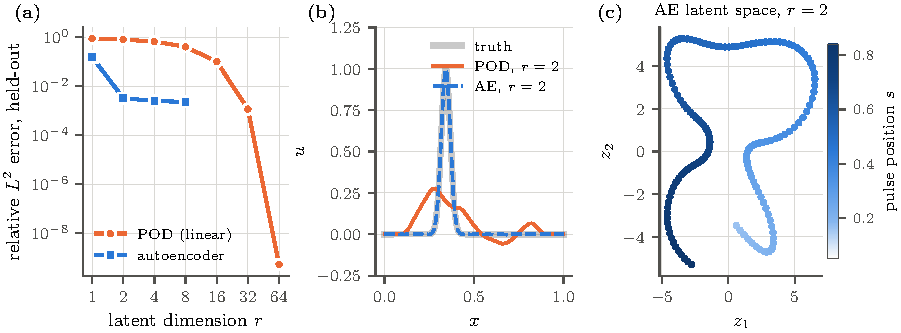
\includegraphics[width=\textwidth]{figs/ae_vs_pod.pdf}
  \caption{Linear versus nonlinear reduction of the advected Gaussian pulse
  (800 training snapshots with random positions, 150 held-out).
  (a)~Held-out relative error of POD and of a fully connected autoencoder
  ($256\!\to\!128\!\to\!64\!\to\!r$, GELU activations; best of three
  initializations) versus latent dimension. (b)~Reconstruction of a held-out
  snapshot with $r=2$. (c)~Latent coordinates of the $r=2$ autoencoder for the
  held-out set, colored by pulse position: the one-parameter family is
  embedded as a smooth curve.}
  \label{fig:ae_vs_pod}
\end{figure}

\subsection{Probabilistic, disentangled, and discrete latent spaces}

The variational autoencoder (VAE) \parencite{kingma2014vae} treats $\z$ as a
random variable with prior $p(\z)=\mathcal{N}(\bm{0},\bm{I})$ and trains an
encoder $q_{\theta}(\z\mid\q)$ and decoder $p_{\vartheta}(\q\mid\z)$ by
maximizing the evidence lower bound. The $\beta$-VAE \parencite{higgins2017betavae}
reweights the Kullback--Leibler term,
\begin{equation}
  \mathcal{L}_{\beta}=\mathbb{E}_{q_{\theta}(\z\mid\q)}\bigl[\log p_{\vartheta}(\q\mid\z)\bigr]
  -\beta\,D_{\mathrm{KL}}\bigl(q_{\theta}(\z\mid\q)\,\|\,p(\z)\bigr),
\end{equation}
and for $\beta>1$ encourages statistically independent, ``disentangled''
latent variables at some cost in reconstruction
\parencite{burgess2018understanding}. In fluids, \textcite{eivazi2022betavae}
used a convolutional $\beta$-VAE to extract a minimal, near-orthogonal set of
nonlinear modes from turbulent flow through a simplified urban environment,
together with an algorithm to rank the modes by contribution.
\textcite{solera2024betavae} combined a $\beta$-VAE with a transformer for a
two-dimensional viscous flow in periodic and chaotic regimes. The
near-orthogonal latent variables resembled POD modes but were more efficient,
and Poincar\'e maps showed that the latent dynamics captured the underlying
attractor. \textcite{wang2024optimal} examined the choice of $\beta$ and latent
dimension for such $\beta$-VAE--transformer models of turbulent flows. The
emphasis of this line of work is the \emph{quality of the latent space for
dynamics} (P3, P6), not reconstruction alone.

Discrete latent spaces are obtained with vector quantization (VQ-VAE)
\parencite{vandenoord2017vqvae}. \textcite{momenifar2022vq} used a
physics-informed VQ model, with incompressibility and velocity-gradient
statistics built into training, to compress DNS data of isotropic turbulence.
Compression for storage is itself an important application.
\textcite{glaws2020insitu} developed an AE for in situ compression of
three-dimensional turbulence. It outperformed a randomized single-pass SVD in
turbulent kinetic energy, enstrophy, and Reynolds stresses at lower cost.
\textcite{mohan2019ccl} combined convolutional compression with a convolutional
LSTM to model three-dimensional turbulence in a compressed space.

\subsection{Choosing the latent dimension}

Unlike POD, an AE provides no spectrum from which to read off a truncation.
Common practice is to scan $r$ and look for a knee in the reconstruction
error, which \textcite{linot2020inertial,linot2022node} used to estimate
inertial-manifold dimensions for the Kuramoto--Sivashinsky equation and
\textcite{linot2023couette} for minimal-flow-unit plane Couette flow at
$\mathrm{Re}=400$. Architectural regularization can make the choice
automatic. The implicit rank-minimizing AE \parencite{jing2020irmae} inserts
linear layers in the bottleneck, which bias training toward low-rank latent
codes. \textcite{zeng2024autoencoders} combined this implicit regularization
with weight decay to estimate the manifold dimension and to produce an
orthogonal manifold coordinate system. Hybrid architectures that first
subtract a PCA projection and learn only a nonlinear correction
\parencite{linot2020inertial} both reduce training cost and make the
linear--nonlinear trade-off explicit.

\subsection{Physics-constrained autoencoders}

Several approaches build physical structure into AEs. Deep Conservation
\parencite{lee2021deepconservation} constrains the latent dynamics so that
the decoded state satisfies conservation laws exactly over subdomains.
\textcite{mohan2020embedding} enforced incompressibility by construction in
convolutional networks for coarse-graining three-dimensional turbulence, using
ideas from numerical methods. Soft constraints in the loss, such as penalties
on mass and momentum conservation \parencite{lee2019cylinder} or on PDE
residuals as in physics-informed neural networks \parencite{raissi2019pinn},
are simpler but guarantee nothing. The manifold Galerkin and LSPG projections
of \textcite{lee2020cae} use the AE only for the representation and enforce the
governing equations in the dynamics, the most direct link between learned
representations and classical ROM theory.

\subsection{Practical considerations}

Deep AEs are the most expressive DR tool in this review, but their advantages
come with costs. (i)~Training is expensive and non-convex; results depend on
architecture, initialization, and optimizer, and should be reported with
variability across seeds. (ii)~Fully connected layers scale with $N$, and
convolutional layers require structured grids. Mesh-agnostic alternatives are
discussed in \cref{sec:meshfree}. (iii)~Reconstruction accuracy saturates, and
small scales are learned last \parencite{rahaman2019spectral}, which matters for
turbulence statistics and spectra. (iv)~Latent coordinates are unique only up
to diffeomorphism, and unordered unless ordering is imposed
\parencite{fukami2020hierarchical,eivazi2022betavae}. (v)~Generalization to
unseen parameters or operating conditions is often the weakest point and
should be tested explicitly (P1). Many of these issues are mitigated by POD
preprocessing \parencite{fresca2022poddlrom} or by hybrid linear--nonlinear
designs \parencite{linot2020inertial}, which suggests that linear and nonlinear
reduction are complementary rather than competing.

% ======================================================================
\section{Mesh-agnostic and operator-based representations}
\label{sec:meshfree}
% ======================================================================

Most methods discussed so far assume that every snapshot lives on the same
discretization, a structured grid in the case of CAEs. Engineering CFD relies on
unstructured, adapted, and moving meshes, and experimental data come on sensor
layouts that change between campaigns. Interpolating such data onto a Cartesian
grid degrades near-wall resolution and couples the learned representation to
an arbitrary choice of grid. This section reviews representations that relax
this assumption, and operator-learning architectures whose internal latent
spaces play the role of a reduced representation.

\subsection{Graph autoencoders}

Graph neural networks operate directly on mesh connectivity. The
encode--process--decode architecture of MeshGraphNets \parencite{pfaff2021meshgraphnets}
showed that message passing on simulation meshes can learn accurate dynamics
for a range of physical systems. It does not, however, reduce the number of
degrees of freedom. Graph autoencoders add pooling (graph coarsening) and
unpooling stages to obtain a genuine bottleneck. \textcite{gruber2022comparison}
found that a graph-convolutional AE is advantageous on data with irregular
connectivity when the latent space is sufficiently large.
\textcite{pichi2024gca} developed graph-convolutional AEs for model order
reduction of parametrized PDEs on unstructured meshes, and
\textcite{barwey2023multiscale} designed multiscale graph AEs whose adaptive
graph-reduction stages identify the spatial regions most relevant to the
dynamics, which provides a form of interpretability. Graph AEs are local by
construction, since each message-passing step aggregates information from a
neighbourhood. They are therefore the unstructured-mesh analogue of both CAEs
and the localized bases of \cref{sec:local}.

\subsection{Implicit neural representations}
\label{sec:inr}

An implicit neural representation (INR), or neural field, represents a flow
field as a coordinate network $\q(\bm{x})\approx g_{\omega}(\bm{x};\z)$
conditioned on a latent code $\z$. Because the decoder can be queried at any
point, the representation is independent of discretization. Encoding is done
either by an encoder network acting on point clouds or by ``auto-decoding'',
which optimizes $\z$ for each snapshot. Coordinate networks suffer severely
from spectral bias, which is mitigated by periodic activations
\parencite{sitzmann2020siren} or random Fourier features \parencite{tancik2020fourier}.

Neural implicit flow (NIF) \parencite{pan2023nif} introduced a mesh-agnostic
DR paradigm for spatio-temporal fluid data. A hypernetwork maps time and
parameters to the weights of a coordinate network, and the hypernetwork
bottleneck serves as the latent space. CROM \parencite{chen2023crom} uses an
INR decoder to build continuous reduced-order models whose latent dynamics
follow from the governing PDE, independent of the training discretization.
DINo \parencite{yin2023dino} evolves the INR latent code with a neural ODE,
giving forecasts that are continuous in space and time. CORAL
\parencite{serrano2023coral} performs operator learning entirely in INR latent
spaces on general geometries. AROMA \parencite{serrano2024aroma} replaces the
single global code with a set of spatially anchored latent tokens decoded by
\emph{local} neural fields and processed by a transformer, so the latent space
preserves spatial structure. This design echoes, in a learned setting, the
local-basis philosophy of DLS. For generative modeling of turbulence,
CoNFiLD \parencite{du2024cnf} trains a latent diffusion model on
conditional-neural-field latents, producing stochastic, spatiotemporally
coherent turbulent fields in irregular geometries.

\subsection{Neural operators and their implicit reduction}

Neural operators learn maps between function spaces
\parencite{kovachki2023neural} and are not usually described as DR methods, yet
most of them contain an explicit or implicit low-dimensional representation.
PCA-Net \parencite{bhattacharya2021pcanet} is explicit: it applies PCA to input
and output functions and learns a map between the coefficients. DeepONet
\parencite{lu2021deeponet} expresses the output as
$\sum_{j=1}^{p}b_j(\text{input})\,t_j(\bm{x})$. Its trunk network $t_j$ is a
learned set of basis functions and its branch network $b_j$ supplies their
coefficients, the same structure as a linear reduced basis with a nonlinear
coefficient map. The Fourier neural operator \parencite{li2021fno} truncates
each layer to a fixed number of Fourier modes, which is a linear spectral
reduction applied repeatedly inside a nonlinear network.
\textcite{kontolati2024latent} made the reduction explicit by training
DeepONets in the latent space of an autoencoder (L-DeepONet), which improved
accuracy and efficiency for high-dimensional, multiscale problems including
fluid flows. Several recent architectures learn \emph{adaptive}
reductions inside attention-based operators. The latent neural operator
\parencite{wang2024lno} maps inputs to a learned latent space by cross-attention.
Transolver \parencite{wu2024transolver} softly assigns mesh points to a small
number of learned ``physical-state slices'' and applies attention among them.
Universal physics transformers \parencite{alkin2024upt} encode arbitrary
particle or mesh data into a fixed set of latent tokens, propagate them, and
decode at arbitrary query points. The distinction between ``dimensionality
reduction followed by a dynamics model'' and ``end-to-end operator learning''
is therefore increasingly one of emphasis. The same questions of latent size,
locality, generalization, and accuracy saturation apply to both.

% ======================================================================
\section{Coupling reduced coordinates to learned dynamics}
\label{sec:dynamics}
% ======================================================================

A reduced representation is rarely an end in itself; in most ML applications it
is the state space of a forecasting or surrogate model. This section surveys
how latent dynamics are learned and, more importantly for the choice of DR,
which properties of the latent space make them learnable.

\subsection{Sequential versus joint training}

In \emph{sequential} training the encoder and decoder are fitted first, by POD,
DLS, or an AE trained on reconstruction alone, and the dynamics model is then
trained on the fixed latent trajectories
\parencite{hasegawa2020bluff,nakamura2021channel,solera2024betavae,morton2026scitech}.
This is modular and cheap, and a single representation can serve several
dynamics models. Reconstruction-optimal coordinates, however, are not
necessarily forecasting-friendly. In \emph{joint} training the dynamics loss is
back-propagated into the encoder, shaping the latent space so that its
evolution is simple: linear \parencite{lusch2018koopman,otto2019linearly},
sparse in a function library \parencite{champion2019sindyae}, or accurately
integrable over several steps \parencite{fresca2021dlrom}. Joint training
couples the design choices and is harder to optimize, but it addresses property
(P3) directly. Intermediate strategies fine-tune a pretrained autoencoder with
a small dynamics loss or add temporal-smoothness regularization to the latent
trajectories.

\subsection{Structured regression: operator inference and sparse identification}

When the latent space is linear (POD), physics suggests the structure of the
reduced model. For the incompressible Navier--Stokes equations Galerkin
projection yields a quadratic system
$\dot{\z}=\bm{c}+\bm{A}\z+\bm{H}(\z\otimes\z)$, and operator inference learns
$\bm{c},\bm{A},\bm{H}$ by least squares from projected trajectories
\parencite{peherstorfer2016opinf,kramer2024opinf}. Lifting transformations
extend this to non-polynomial systems \parencite{qian2020liftlearn}, and
quadratic manifolds extend it to curved trial manifolds
\parencite{geelen2023quadratic}. Sparse identification of nonlinear dynamics
(SINDy) \parencite{brunton2016sindy} instead selects a few terms from a library
of candidate functions by sparse regression, yielding interpretable latent
equations. \textcite{loiseau2018sparse} applied it to sensor-derived features.
\textcite{champion2019sindyae} trained an autoencoder jointly with a SINDy model
so that the discovered coordinates admit a parsimonious governing equation.
The LaSDI family extends this to parametric problems: latent ODE coefficients
are identified for each training parameter and interpolated to new ones
\parencite{fries2022lasdi}, with greedy, physics-informed sampling of training
parameters \parencite{he2023glasdi} and Gaussian-process interpolation with
uncertainty quantification \parencite{bonneville2024gplasdi}.

\subsection{Koopman embeddings}
\label{sec:koopman}

Koopman operator theory seeks observables in which a nonlinear system evolves
linearly \parencite{mezic2013,brunton2022koopman}. Deep Koopman methods learn
these observables with an autoencoder and impose linear latent dynamics
$\z_{k+1}=\bm{K}\z_k$ through a multi-step prediction loss
\parencite{takeishi2017koopman,lusch2018koopman,otto2019linearly}.
\textcite{lusch2018koopman} used an auxiliary network to parametrize eigenvalues
as functions of the state, capturing systems with continuous spectra.
\textcite{morton2018deep} learned such models of cylinder-wake dynamics and
used them for model-predictive control, and \textcite{pan2020physics}
introduced a probabilistic formulation with guaranteed stability. For a
low-order model of near-wall turbulence, \textcite{eivazi2021koopman} found that
a Koopman framework with nonlinear forcing reproduced the long-term statistics
as accurately as an LSTM at lower cost, and gave better short-term
predictions. Koopman embeddings also serve as tokenizers for transformers
\parencite{geneva2022transformers}.

\subsection{Recurrent networks, reservoir computing, and neural ODEs}

Recurrent networks, especially LSTMs \parencite{hochreiter1997lstm}, were the
first widely used black-box latent dynamics models.
\textcite{vlachas2018lstm} forecast high-dimensional chaotic systems with LSTMs
in a reduced-order space. For the nine-equation model of turbulent shear flow,
\textcite{srinivasan2019} reproduced turbulence statistics with sub-percent
errors using LSTMs. The LSTM-on-POD and LSTM-on-CAE combinations of
\cref{sec:pod,sec:autoencoders} follow the same pattern
\parencite{wang2018model,mohan2018lstm,eivazi2020deep,hasegawa2020bluff,maulik2021advection,borrelli2022channels}.
Reservoir computing trains only a linear readout of a large random recurrent
network. It forecasts spatiotemporal chaos well when combined with spatial
localization \parencite{pathak2018reservoir} or with a CAE latent space
\parencite{racca2023caesn}, and \textcite{vlachas2020backprop} compared it
systematically with back-propagated RNNs. Neural ODEs \parencite{chen2018node}
learn a continuous-time vector field $\dot{\z}=\bm{f}_{\theta}(\z)$, which
suits irregularly sampled data and connects naturally with dynamical-systems
analysis. In autoencoder coordinates of the Kuramoto--Sivashinsky equation,
\textcite{linot2022node} found that dimension reduction improves performance
relative to learning in the ambient space, and identified a ``sweet spot''
in latent dimension. Stabilized variants add a learned linear damping term for
long-time forecasting \parencite{linot2023stabilized}, and the approach has been
applied to minimal-flow-unit Couette turbulence \parencite{linot2023couette}.
Learning the effective dynamics (LED) \parencite{vlachas2022led} couples an AE
and a recurrent latent propagator with intermittent fine-scale simulation in
an equation-free framework, reducing computational effort by up to two orders
of magnitude while maintaining accuracy.

\subsection{Attention-based sequence models}

Transformers \parencite{vaswani2017attention} replace recurrence with
self-attention over a context window of past latent states, which captures
long-range temporal dependencies and trains in parallel.
\textcite{wu2022transformer} combined a transformer with POD for flows past a
cylinder and a group of buildings, and \textcite{geneva2022transformers} with
Koopman embeddings for several physical systems. \textcite{hemmasian2023transformers}
used a CAE latent space and reported competitive results even for turbulent
datasets. \textcite{solera2024betavae} and \textcite{wang2024optimal} used
$\beta$-VAE latent spaces. Transformers have also been used without a
separate autoencoder, on subsampled or pre-processed fields:
\textcite{yousif2023transformer} generated turbulent inflow planes for
spatially developing boundary layers by combining a transformer with a
super-resolution GAN, and \textcite{sarma2024tbl} predicted actuated turbulent
boundary-layer fields after a dimensionality-reducing pre-processing step.
\textcite{morton2026scitech} paired transformers with DLS latent spaces for
cavity flows at $\mathrm{Re}=15{,}000$ and $30{,}000$
(\cref{sec:dls}). Attention can also operate over \emph{space}: when the latent
state is a set of spatially anchored tokens, as in DLS, AROMA, or universal
physics transformers
\parencite{deshmukh2020dls,serrano2024aroma,alkin2024upt}, the sequence model can
attend across tokens as well as time, and forecasting itself can be posed
locally.

\subsection{Latent generative models}

Deterministic models trained with a mean-squared loss converge to the
conditional mean of future states. For chaotic flows this is smoother and less
energetic than any single realization, and the resulting under-dispersion
often drives rollout drift. Generative models address this by learning the
distribution of future states. Latent diffusion models, developed for images
\parencite{rombach2022ldm}, have been adapted to turbulence generation with
conditional-neural-field latents \parencite{du2024cnf} and to Bayesian
conditional generation \parencite{gao2024bayesian}. \textcite{kohl2023acdm}
benchmarked autoregressive conditional diffusion models for turbulent flow
prediction. Even simple diffusion approaches matched or outperformed
established methods in accuracy and temporal stability, at a higher inference
cost, while providing samples consistent with the flow statistics. PDE-Refiner
\parencite{lippe2023pderefiner} achieves accurate long rollouts through an
iterative refinement that attends to low-amplitude frequency components. The
compression provided by DR is especially valuable for diffusion models, whose
cost scales with the dimension of the space in which they denoise.

\subsection{What makes a latent space good for dynamics?}
\label{sec:goodlatent}

Across these studies, several latent-space properties recur as predictors of
successful forecasting, beyond reconstruction accuracy.
\begin{itemize}[leftmargin=1.5em,itemsep=2pt]
  \item \emph{Sufficiency and Markovianity.} The latent state must retain
  enough information to determine its own future. Aggressive truncation removes
  small scales that feed back on large ones, so the latent dynamics become
  non-Markovian. This is the origin of the closure problem in POD--Galerkin
  models \parencite{wang2012closure,ahmed2021closures}, and it appears in
  learned models as the need for long input histories or memory terms
  \parencite{maulik2020timeseries}.
  \item \emph{Smoothness and low temporal complexity.} Latent coordinates that
  vary smoothly and with few dominant frequencies are easier to forecast.
  Near-orthogonal, disentangled coordinates
  \parencite{eivazi2022betavae,solera2024betavae} and ordered coordinates
  \parencite{fukami2020hierarchical} were motivated partly by this. Localized
  coordinates may reduce temporal complexity in a different way: each local
  coefficient reflects only nearby structures, so its time series can carry a
  narrower range of scales than a global mode that mixes contributions from
  the whole domain. This is one motivation for the localized latent spaces of
  \textcite{morton2026scitech}.
  \item \emph{Appropriate dimension.} Too small a latent space discards
  dynamics, and too large a space adds noisy, weakly constrained directions in
  which errors grow; \textcite{linot2022node} found an intermediate optimum.
  \item \emph{Stability.} Latent spaces or dynamics models with built-in
  stability \parencite{pan2020physics,linot2023stabilized}, and training on
  multi-step rollouts instead of single steps
  \parencite{lusch2018koopman,kohl2023acdm}, reduce error accumulation.
  \item \emph{Statistical fidelity.} For turbulence, matching second-order
  statistics and spectra matters as much as pointwise accuracy, which favours
  representations that retain small-scale energy
  \parencite{deshmukh2018energy,glaws2020insitu} and training objectives or
  generative models that do not collapse to the conditional mean
  \parencite{kohl2023acdm,du2024cnf}.
\end{itemize}

% ======================================================================
\section{Comparative assessment}
\label{sec:assessment}
% ======================================================================

\subsection{Summary of properties}

\Cref{tab:summary} summarizes the families reviewed above against the
properties (P1)--(P7) of \cref{sec:desiderata}. The entries are qualitative and
reflect typical behaviour reported in the literature and in our computed
examples; any given implementation can do better or worse.

\begin{table}[tbp]
\centering
\caption{Qualitative comparison of dimensionality reduction families for
fluid-dynamics machine learning. Columns: \emph{Dec.}\ explicit, cheap decoder;
\emph{Transp.}\ latent size needed for transport-dominated or multi-scale flows
(slowly decaying Kolmogorov $n$-width); \emph{Data} number of snapshots needed
to build the representation; \emph{Scal.}\ cost and memory for large $N$ and
mesh flexibility; \emph{Interp.}\ interpretability; \emph{Acc.}\ attainable
accuracy as the latent size grows. $+$ favourable, $\circ$ intermediate,
$-$ unfavourable.}
\label{tab:summary}
\footnotesize
\setlength{\tabcolsep}{3pt}
\renewcommand{\arraystretch}{1.15}
\begin{tabularx}{\textwidth}{@{}>{\raggedright\arraybackslash}p{4.3cm} *{6}{c} >{\raggedright\arraybackslash}X@{}}
\toprule
Family & Dec. & Transp. & Data & Scal. & Interp. & Acc. & Representative fluid uses \\
\midrule
POD / PCA & $+$ & $-$ & $\circ$ & $+$ & $+$ & $+$ & Galerkin ROMs, POD--LSTM/transformer, OpInf \\
DMD, SPOD, balanced POD & $+$ & $-$ & $\circ$ & $+$ & $+$ & $+$ & Modal analysis, Koopman models, control \\
Transport-adapted linear & $+$ & $\circ$ & $\circ$ & $\circ$ & $+$ & $+$ & Shocks, fronts, traveling waves \\
Sparse, clustered, local ROBs & $\circ$ & $\circ$ & $\circ$ & $\circ$ & $+$ & $+$ & Multi-scale Galerkin ROMs, regime switching \\
Domain decomposition, GFEM, DLS & $+$ & $\circ$ & $+$ & $+$ & $+$ & $+$ & Extreme-scale ROMs, turbulent latent spaces \\
Kernel / graph manifold learning & $-$ & $+$ & $\circ$ & $-$ & $\circ$ & $\circ$ & Manifold identification, regime analysis \\
Quadratic manifolds & $+$ & $\circ$ & $\circ$ & $+$ & $\circ$ & $+$ & Projection ROMs beyond linear subspaces \\
MLP / convolutional AE & $+$ & $+$ & $-$ & $\circ$ & $-$ & $-$ & Nonlinear ROMs, AE--LSTM/transformer \\
VAE, $\beta$-VAE, VQ-VAE & $+$ & $+$ & $-$ & $\circ$ & $\circ$ & $-$ & Disentangled modes, compression, generation \\
Graph autoencoders & $+$ & $+$ & $-$ & $\circ$ & $\circ$ & $-$ & Unstructured meshes \\
Implicit neural representations & $+$ & $+$ & $-$ & $\circ$ & $-$ & $-$ & Mesh-agnostic ROMs, generative turbulence \\
Latent neural operators & $+$ & $+$ & $-$ & $\circ$ & $-$ & $-$ & Parametric surrogates, general geometries \\
\bottomrule
\end{tabularx}
\end{table}

Two broad patterns emerge. First, representations with linear, explicit
encoders and decoders (POD, DMD, GFEM/DLS) are cheap, reproducible, and reach
arbitrarily high accuracy as the latent size grows. They are the natural choice
when training data are limited or when accuracy of small scales matters.
Learned nonlinear decoders achieve much smaller latent spaces for
transport-dominated and low-intrinsic-dimension problems but saturate in
accuracy and require more data and tuning. Second, the right choice depends on
the \emph{flow}, not only on the method. \Cref{fig:ldc_pod} shows that the
$\mathrm{Re}=15{,}000$ cavity is dominated by a few coherent modes, so global
POD is close to optimal for reconstructing it at a fixed latent size
(\cref{fig:dls_compare}a). The same is not true for the advected pulse of
\cref{fig:nwidth,fig:ae_vs_pod} or, by extension, for strongly convective or
broadband turbulent flows.

\subsection{Evidence from comparative studies}

Systematic comparisons remain scarce, and their conclusions are nuanced.
\textcite{csala2022comparing} and \textcite{mendez2023linear} found that
nonlinear methods can represent canonical flows with fewer coordinates than
PCA, but that the advantage depends on the flow, the arrangement of the data,
and the task (filtering, pattern identification, or compression).
\textcite{gruber2022comparison} showed that no single autoencoder architecture
dominates: the best choice depends on latent size and data structure.
\textcite{swischuk2019projection} compared several regression methods on POD
coefficients and argued for retaining the projection structure.
\textcite{fresca2022poddlrom} showed that a linear POD stage before the
autoencoder reduces training cost substantially without sacrificing accuracy.
For forecasting, \textcite{eivazi2021koopman} found a Koopman framework as
accurate as an LSTM in long-term statistics at lower cost, and
\textcite{morton2026scitech} found that transformers performed well on a
localized DLS latent space but poorly on a POD latent space of the same flow.
A common thread is that linear and nonlinear, global and local
representations are complementary. Hybrids that combine a linear or local
backbone with nonlinear corrections often perform best
\parencite{linot2020inertial,fresca2022poddlrom,diaz2024ddnm}.

\subsection{Baselines, benchmarks, and metrics}

\textcite{mcgreivy2024weak} documented that weak baselines and reporting biases
lead to systematic over-optimism in ML for fluid-related PDEs. For DR the
corresponding risks are comparing a tuned nonlinear model against an untuned
linear one, reporting training rather than held-out error, and choosing
latent sizes that favour one method. Based on the studies reviewed here, we
recommend the following practices.
\begin{enumerate}[leftmargin=2em,itemsep=2pt]
  \item Always report a POD baseline at the \emph{same} latent dimension and,
  for dynamics, a POD--based model with the same sequence architecture. Report
  POD error as a function of $r$, not at a single truncation.
  \item Evaluate reconstruction on held-out data that are separated in time
  from the training data and, where relevant, at unseen parameters or
  operating conditions (P1). Report training-data requirements (P4) alongside
  accuracy, as in \cref{fig:dls_compare}b.
  \item Report the full storage cost (latent coefficients \emph{and} basis or
  network parameters) when claiming compression, and the latent dimension seen
  by the dynamics model when claiming learnability.
  \item Beyond pointwise error, report second-order statistics (Reynolds
  stresses, turbulent kinetic energy), spectra, and, for forecasts, long-time
  statistics and error growth over rollouts. Small-scale fidelity is where
  methods differ most.
  \item Report variability over random initializations for learned
  representations.
\end{enumerate}
Common benchmark resources support such comparisons. They include the
Johns Hopkins turbulence databases \parencite{li2008jhtdb}, PDEBench
\parencite{takamoto2022pdebench}, The Well \parencite{ohana2024well}, and the
community challenge of \textcite{schmidt2026challenge}. The last has
separate tracks for compression, forecasting, and sensing of aerospace flows,
among them experimental time-resolved PIV of a Mach 0.6 cavity flow of the type
analysed by \textcite{zhang2020samm}.

\subsection{Practical guidance}

The choice of representation can be organized around four questions.
\begin{enumerate}[leftmargin=2em,itemsep=2pt]
  \item \emph{How fast does the POD spectrum decay?} If a few percent of the
  snapshots' rank captures the required energy on held-out data, POD (or DMD
  or SPOD for spectral content) is hard to beat and should be the default.
  \item \emph{Is the difficulty transport or multi-scale content?} Transport of a
  few coherent features favours transport-adapted linear methods or nonlinear
  autoencoders with small latent spaces. Broadband, multi-scale content over a
  large domain favours localized representations (domain decomposition, DLS,
  graph or local-token architectures) whose cost grows with the domain rather
  than with the number of distinct global patterns.
  \item \emph{How much data is there, and on what discretization?} Limited
  snapshots favour linear and local bases, since local bases draw many
  training samples from each snapshot. Unstructured or changing
  discretizations favour graph AEs and implicit neural representations.
  \item \emph{What will the latent space be used for?} Galerkin projection
  needs an explicit, differentiable decoder; control benefits from balanced or
  Koopman coordinates; long-horizon forecasting benefits from smooth,
  Markovian, and possibly localized coordinates; and generative modeling
  benefits from compact, well-regularized latent spaces.
\end{enumerate}

% ======================================================================
\section{Open challenges and outlook}
\label{sec:outlook}
% ======================================================================

\paragraph{Scaling to high-Reynolds-number, three-dimensional flows.}
Most demonstrations of learned representations use two-dimensional or
low-Reynolds-number flows, for which global bases or small autoencoders
suffice. Operationally relevant flows are different in kind. Ship airwakes,
for example, are massively separated flows at Reynolds numbers of order
$10^{7}$--$10^{8}$ that must be predicted over many wind-over-deck conditions
for flight simulation and flight-deck safety analysis
\parencite{polsky2016safedi}. At this scale even storing global snapshots
strains memory, dense encoders are infeasible, and the number of
distinct flow patterns grows with domain size and Reynolds number.
Representations whose cost and training data grow with the \emph{local}
complexity of the flow rather than its global complexity are therefore
attractive. These include domain-decomposed and GFEM-enriched bases
\parencite{hoang2021ddlspg,diaz2024ddnm,deshmukh2020dls}, graph and
local-token architectures \parencite{barwey2023multiscale,serrano2024aroma},
and in situ compression \parencite{glaws2020insitu}. Whether forecasting
itself can be posed locally without losing long-range coupling is an open
question. So is how locality interacts with the global pressure field of
incompressible flow.

\paragraph{Generalization across parameters and conditions.}
Interpolating between training parameters works well for smooth parametric
dependence \parencite{amsallem2008grassmann,fries2022lasdi}, but extrapolation to
new geometries, Reynolds numbers, or operating conditions remains the weakest
point of learned representations. Local bases may generalize better because
local flow features (shear layers, boundary layers, vortices) recur across
conditions even when their global arrangement changes. This hypothesis
deserves systematic testing.

\paragraph{Experimental and sparse data.}
Experimental data are noisy, gappy, and often not time-resolved. Classical
tools include gappy POD \parencite{everson1995gappy}, spectral estimation from
non-time-resolved PIV synchronized with pressure sensors
\parencite{zhang2020samm}, and sparse-sensor reconstruction
\parencite{manohar2018sensor,callaham2019robust,erichson2020shallow}. They need to
be integrated with learned representations, for example by training encoders
that accept partial observations or by using generative latent models for
conditional reconstruction \parencite{du2024cnf}.

\paragraph{Uncertainty, statistics, and generative modeling.}
For chaotic flows, point forecasts beyond a few Lyapunov times are
meaningless. What matters is whether a model reproduces the statistics and the
distribution of future states. Probabilistic latent spaces and latent
diffusion models \parencite{kohl2023acdm,gao2024bayesian,du2024cnf} are promising
but expensive, and their evaluation calls for statistical and spectral metrics
rather than pointwise error.

\paragraph{Interpretability and physical consistency.}
Linear and local bases offer interpretable modes and simple error estimates.
Learned representations offer compactness at the cost of both. Continued work
on ordered and disentangled latent variables
\parencite{fukami2020hierarchical,eivazi2022betavae}, on relating latent
coordinates to invariant solutions and physical mechanisms
\parencite{page2021revealing,farzamnik2023snapshots}, and on hard physical
constraints \parencite{lee2021deepconservation,mohan2020embedding} will be needed
before learned representations are trusted in engineering practice.

\paragraph{Foundation models and tokenization.}
Pretrained models for PDEs \parencite{mccabe2024mpp,herde2024poseidon} and large
multi-physics data collections \parencite{ohana2024well} raise a new version of
the representation question: how should heterogeneous flow data be tokenized?
Patch tokens \parencite{dosovitskiy2021vit}, learned slices
\parencite{wu2024transolver}, latent tokens \parencite{alkin2024upt}, and
physically structured local bases \parencite{deshmukh2020dls} embody different
answers. The DR literature reviewed here, with its emphasis on optimality,
locality, and multi-scale structure, is directly relevant to that choice.

% ======================================================================
\section{Conclusions}
\label{sec:conclusions}
% ======================================================================

Dimensionality reduction is the foundation on which data-driven models of
fluid flows are built. It fixes the information available to the dynamics
model, the cost of training and inference, and the difficulty of the learning
problem. Linear modal decompositions remain the indispensable baseline: they are
optimal among linear subspaces, cheap, interpretable, and, for flows dominated
by a few coherent structures, hard to beat. Their limitations for transport and
multi-scale turbulence are well understood through the Kolmogorov $n$-width.
Two broad responses have emerged. Nonlinear manifold methods, from kernel and
graph embeddings to deep and variational autoencoders and implicit neural
representations, achieve compact latent spaces when the intrinsic dimension is
low, at the cost of data, tuning, and an accuracy ceiling. Localized
representations, from domain decomposition to GFEM enrichment and data-informed
local subspaces, keep linear, sparse encoders and decoders with guaranteed
continuity. They learn from few snapshots and scale with the local rather than
global complexity of the flow, at the cost of larger latent spaces when the
flow is globally simple.

The literature increasingly suggests that these choices are complementary,
and that representations should be judged by how well they support learning
the dynamics: whether the latent state is sufficient, smooth, stable, and
statistically faithful, not only by reconstruction error. Progress toward
high-Reynolds-number, three-dimensional, and parametrically varying flows of
engineering interest will depend on representations that respect the
multi-scale and local structure of turbulence. It will also depend on
evaluation against strong baselines, held-out conditions, and statistical
metrics.


\section*{Reproducibility of figures}
\addcontentsline{toc}{section}{Reproducibility of figures}
All computed figures were generated by the scripts in \texttt{code/}.
\Cref{fig:ldc_pod,fig:dls_compare,fig:dls_recon} use the $\mathrm{Re}=15{,}000$
lid-driven cavity dataset (\texttt{ldc\_15k.h5}) and, for the DLS results, the
project implementation of the generalized finite element compressor
(\texttt{lib/dls\_2d.py}).
\Cref{fig:nwidth,fig:ae_vs_pod} are self-contained one-dimensional experiments.
The bibliography was checked against the Crossref and DataCite registries
(\texttt{code/verify\_bib.py}).

\printbibliography[heading=bibintoc,title={References}]

\end{document}
